%%%%%%%%%%%%%%%%%%%%%%%%%%%%%%%%%%%%%%%%%
% The Legrand Orange Book
% LaTeX Template
% Version 2.2 (30/3/17)
%
% This template has been downloaded from:
% http://www.LaTeXTemplates.com
%
% Original author:
% Mathias Legrand (legrand.mathias@gmail.com) with modifications by:
% Vel (vel@latextemplates.com)
%
% License:
% CC BY-NC-SA 3.0 (http://creativecommons.org/licenses/by-nc-sa/3.0/)
%
% Compiling this template:
% This template uses biber for its bibliography and makeindex for its index.
% When you first open the template, compile it from the command line with the 
% commands below to make sure your LaTeX distribution is configured correctly:
%
% 1) pdflatex main
% 2) makeindex main.idx -s StyleInd.ist
% 3) biber main
% 4) pdflatex main x 2
%
% After this, when you wish to update the bibliography/index use the appropriate
% command above and make sure to compile with pdflatex several times 
% afterwards to propagate your changes to the document.
%
% This template also uses a number of packages which may need to be
% updated to the newest versions for the template to compile. It is strongly
% recommended you update your LaTeX distribution if you have any
% compilation errors.
%
% Important note:
% Chapter heading images should have a 2:1 width:height ratio,
% e.g. 920px width and 460px height.
%
%%%%%%%%%%%%%%%%%%%%%%%%%%%%%%%%%%%%%%%%%

%----------------------------------------------------------------------------------------
%	PACKAGES AND OTHER DOCUMENT CONFIGURATIONS
%----------------------------------------------------------------------------------------

\documentclass[11pt,fleqn]{book} % Default font size and left-justified equations

%----------------------------------------------------------------------------------------

%%%%%%%%%%%%%%%%%%%%%%%%%%%%%%%%%%%%%%%%%
% The Legrand Orange Book
% Structural Definitions File
% Version 2.0 (9/2/15)
%
% Original author:
% Mathias Legrand (legrand.mathias@gmail.com) with modifications by:
% Vel (vel@latextemplates.com)
% 
% This file has been downloaded from:
% http://www.LaTeXTemplates.com
%
% License:
% CC BY-NC-SA 3.0 (http://creativecommons.org/licenses/by-nc-sa/3.0/)
%
%%%%%%%%%%%%%%%%%%%%%%%%%%%%%%%%%%%%%%%%%

%----------------------------------------------------------------------------------------
%	VARIOUS REQUIRED PACKAGES AND CONFIGURATIONS
%----------------------------------------------------------------------------------------
%	PAQUETES PERSONALES
%----------------------------------------------------------------------------------------
\usepackage{graphicx}
\usepackage[dvipsnames]{xcolor}
\usepackage{colortbl}
\usepackage{listings}
\usepackage{float}
\usepackage{color}
\usepackage{enumerate}
%\textsl{}
%----------------------------------------------------------------------------------------
%PAQUETES NECESARIOS
%----------------------------------------------------------------------------------------
\usepackage[top=3cm,bottom=3cm,left=3cm,right=3cm,headsep=10pt,a4paper]{geometry} % Page margins
\usepackage{graphicx} % Required for including pictures
\graphicspath{{CabecerasCapitulos/}} % Specifies the directory where pictures are stored
\usepackage{lipsum} % Inserts dummy text
\usepackage{tikz} % Required for drawing custom shapes
\usepackage[spanish]{babel} % English language/hyphenation
\usepackage{enumitem} % Customize lists
\setlist{nolistsep} % Reduce spacing between bullet points and numbered lists
\usepackage{booktabs} % Required for nicer horizontal rules in tables
\usepackage{xcolor} % Required for specifying colors by name
\definecolor{blue}{RGB}{74,136,229} % Define the orange color used for highlighting throughout the book

%----------------------------------------------------------------------------------------
%	FONTS
%----------------------------------------------------------------------------------------

\usepackage{avant} % Use the Avantgarde font for headings
%\usepackage{times} % Use the Times font for headings
\usepackage{mathptmx} % Use the Adobe Times Roman as the default text font together with math symbols from the Sym­bol, Chancery and Com­puter Modern fonts
\usepackage{microtype} % Slightly tweak font spacing for aesthetics
\usepackage[utf8]{inputenc} % Required for including letters with accents
\usepackage[T1]{fontenc} % Use 8-bit encoding that has 256 glyphs

%----------------------------------------------------------------------------------------
%	BIBLIOGRAPHY AND INDEX
%----------------------------------------------------------------------------------------
%backend=biber/bibtex
%style=numeric/alphabetic
%citestyle=numeric/authoryear
\usepackage[style=numeric,citestyle=numeric,sorting=nyt,sortcites=true,autopunct=true,babel=hyphen,hyperref=true,abbreviate=false,backref=true,backend=bibtex]{biblatex}
\addbibresource{Referencias/bibliography.bib} % BibTeX bibliography file
%\addbibresource{una por una ref.ext}
\defbibheading{bibempty}{}
\usepackage{calc} % For simpler calculation - used for spacing the index letter headings correctly
\usepackage{makeidx} % Required to make an index
\makeindex % Tells LaTeX to create the files required for indexing
%----------------------------------------------------------------------------------------
%	MAIN TABLE OF CONTENTS
%----------------------------------------------------------------------------------------

\usepackage{titletoc} % Required for manipulating the table of contents

\contentsmargin{0cm} % Removes the default margin

% Part text styling
\titlecontents{part}[0cm]
{\addvspace{20pt}\centering\large\bfseries}
{}
{}
{}

% Chapter text styling
\titlecontents{chapter}[1.25cm] % Indentation
{\addvspace{12pt}\large\sffamily\bfseries} % Spacing and font options for chapters
{\color{blue!60}\contentslabel[\Large\thecontentslabel]{1.25cm}\color{blue}} % Chapter number
{\color{blue}}  
{\color{blue!60}\normalsize\;\titlerule*[.5pc]{.}\;\thecontentspage} % Page number

% Section text styling
\titlecontents{section}[1.25cm] % Indentation
{\addvspace{3pt}\sffamily\bfseries} % Spacing and font options for sections
{\contentslabel[\thecontentslabel]{1.25cm}} % Section number
{}
{\hfill\color{black}\thecontentspage} % Page number
[]

% Subsection text styling
\titlecontents{subsection}[1.25cm] % Indentation
{\addvspace{1pt}\sffamily\small} % Spacing and font options for subsections
{\contentslabel[\thecontentslabel]{1.25cm}} % Subsection number
{}
{\ \titlerule*[.5pc]{.}\;\thecontentspage} % Page number
[]

% List of figures
\titlecontents{figure}[0em]
{\addvspace{-5pt}\sffamily}
{\thecontentslabel\hspace*{1em}}
{}
{\ \titlerule*[.5pc]{.}\;\thecontentspage}
[]

% List of tables
\titlecontents{table}[0em]
{\addvspace{-5pt}\sffamily}
{\thecontentslabel\hspace*{1em}}
{}
{\ \titlerule*[.5pc]{.}\;\thecontentspage}
[]

%----------------------------------------------------------------------------------------
%	MINI TABLE OF CONTENTS IN PART HEADS
%----------------------------------------------------------------------------------------

% Chapter text styling
\titlecontents{lchapter}[0em] % Indenting
{\addvspace{15pt}\large\sffamily\bfseries} % Spacing and font options for chapters
{\color{blue}\contentslabel[\Large\thecontentslabel]{1.25cm}\color{blue}} % Chapter number
{}  
{\color{blue}\normalsize\sffamily\bfseries\;\titlerule*[.5pc]{.}\;\thecontentspage} % Page number

% Section text styling
\titlecontents{lsection}[0em] % Indenting
{\sffamily\small} % Spacing and font options for sections
{\contentslabel[\thecontentslabel]{1.25cm}} % Section number
{}
{}

% Subsection text styling
\titlecontents{lsubsection}[.5em] % Indentation
{\normalfont\footnotesize\sffamily} % Font settings
{}
{}
{}

%----------------------------------------------------------------------------------------
%	PAGE HEADERS
%----------------------------------------------------------------------------------------

\usepackage{fancyhdr} % Required for header and footer configuration

\pagestyle{fancy}
\renewcommand{\chaptermark}[1]{\markboth{\sffamily\normalsize\bfseries\chaptername\ \thechapter.\ #1}{}} % Chapter text font settings
\renewcommand{\sectionmark}[1]{\markright{\sffamily\normalsize\thesection\hspace{5pt}#1}{}} % Section text font settings
\fancyhf{} \fancyhead[LE,RO]{\sffamily\normalsize\thepage} % Font setting for the page number in the header
\fancyhead[LO]{\rightmark} % Print the nearest section name on the left side of odd pages
\fancyhead[RE]{\leftmark} % Print the current chapter name on the right side of even pages
\renewcommand{\headrulewidth}{0.5pt} % Width of the rule under the header
\addtolength{\headheight}{2.5pt} % Increase the spacing around the header slightly
\renewcommand{\footrulewidth}{0pt} % Removes the rule in the footer
\fancypagestyle{plain}{\fancyhead{}\renewcommand{\headrulewidth}{0pt}} % Style for when a plain pagestyle is specified

% Removes the header from odd empty pages at the end of chapters
\makeatletter
\renewcommand{\cleardoublepage}{
\clearpage\ifodd\c@page\else
\hbox{}
\vspace*{\fill}
\thispagestyle{empty}
\newpage
\fi}

%----------------------------------------------------------------------------------------
%	THEOREM STYLES
%----------------------------------------------------------------------------------------

\usepackage{amsmath,amsfonts,amssymb,amsthm} % For math equations, theorems, symbols, etc

\newcommand{\intoo}[2]{\mathopen{]}#1\,;#2\mathclose{[}}
\newcommand{\ud}{\mathop{\mathrm{{}d}}\mathopen{}}
\newcommand{\intff}[2]{\mathopen{[}#1\,;#2\mathclose{]}}
\newtheorem{notation}{Notation}[chapter]

% Boxed/framed environments
\newtheoremstyle{ocrenumbox}% % Theorem style name
{0pt}% Space above
{0pt}% Space below
{\normalfont}% % Body font
{}% Indent amount
{\small\bf\sffamily\color{blue}}% % Theorem head font
{\;}% Punctuation after theorem head
{0.25em}% Space after theorem head
{\small\sffamily\color{blue}\thmname{#1}\nobreakspace\thmnumber{\@ifnotempty{#1}{}\@upn{#2}}% Theorem text (e.g. Theorem 2.1)
\thmnote{\nobreakspace\the\thm@notefont\sffamily\bfseries\color{black}---\nobreakspace#3.}} % Optional theorem note
\renewcommand{\qedsymbol}{$\blacksquare$}% Optional qed square

\newtheoremstyle{blacknumex}% Theorem style name
{5pt}% Space above
{5pt}% Space below
{\normalfont}% Body font
{} % Indent amount
{\small\bf\sffamily}% Theorem head font
{\;}% Punctuation after theorem head
{0.25em}% Space after theorem head
{\small\sffamily{\tiny\ensuremath{\blacksquare}}\nobreakspace\thmname{#1}\nobreakspace\thmnumber{\@ifnotempty{#1}{}\@upn{#2}}% Theorem text (e.g. Theorem 2.1)
\thmnote{\nobreakspace\the\thm@notefont\sffamily\bfseries---\nobreakspace#3.}}% Optional theorem note

\newtheoremstyle{blacknumbox} % Theorem style name
{0pt}% Space above
{0pt}% Space below
{\normalfont}% Body font
{}% Indent amount
{\small\bf\sffamily}% Theorem head font
{\;}% Punctuation after theorem head
{0.25em}% Space after theorem head
{\small\sffamily\thmname{#1}\nobreakspace\thmnumber{\@ifnotempty{#1}{}\@upn{#2}}% Theorem text (e.g. Theorem 2.1)
\thmnote{\nobreakspace\the\thm@notefont\sffamily\bfseries---\nobreakspace#3.}}% Optional theorem note

% Non-boxed/non-framed environments
\newtheoremstyle{ocrenum}% % Theorem style name
{5pt}% Space above
{5pt}% Space below
{\normalfont}% % Body font
{}% Indent amount
{\small\bf\sffamily\color{blue}}% % Theorem head font
{\;}% Punctuation after theorem head
{0.25em}% Space after theorem head
{\small\sffamily\color{blue}\thmname{#1}\nobreakspace\thmnumber{\@ifnotempty{#1}{}\@upn{#2}}% Theorem text (e.g. Theorem 2.1)
\thmnote{\nobreakspace\the\thm@notefont\sffamily\bfseries\color{black}---\nobreakspace#3.}} % Optional theorem note
\renewcommand{\qedsymbol}{$\blacksquare$}% Optional qed square
\makeatother

% Defines the theorem text style for each type of theorem to one of the three styles above
\newcounter{dummy} 
\numberwithin{dummy}{section}
\theoremstyle{ocrenumbox}
\newtheorem{theoremeT}[dummy]{Theorem}
\newtheorem{problem}{Problem}[chapter]
\newtheorem{exerciseT}{Exercise}[chapter]
\theoremstyle{blacknumex}
\newtheorem{exampleT}{Example}[chapter]
\theoremstyle{blacknumbox}
\newtheorem{vocabulary}{Vocabulary}[chapter]
\newtheorem{definitionT}{Definition}[section]
\newtheorem{corollaryT}[dummy]{Corollary}
\theoremstyle{ocrenum}
\newtheorem{proposition}[dummy]{Proposition}

%----------------------------------------------------------------------------------------
%	DEFINITION OF COLORED BOXES
%----------------------------------------------------------------------------------------

\RequirePackage[framemethod=default]{mdframed} % Required for creating the theorem, definition, exercise and corollary boxes

% Theorem box
\newmdenv[skipabove=7pt,
skipbelow=7pt,
backgroundcolor=black!5,
linecolor=blue,
innerleftmargin=5pt,
innerrightmargin=5pt,
innertopmargin=5pt,
leftmargin=0cm,
rightmargin=0cm,
innerbottommargin=5pt]{tBox}

% Exercise box	  
\newmdenv[skipabove=7pt,
skipbelow=7pt,
rightline=false,
leftline=true,
topline=false,
bottomline=false,
backgroundcolor=blue!10,
linecolor=blue,
innerleftmargin=5pt,
innerrightmargin=5pt,
innertopmargin=5pt,
innerbottommargin=5pt,
leftmargin=0cm,
rightmargin=0cm,
linewidth=4pt]{eBox}	

% Definition box
\newmdenv[skipabove=7pt,
skipbelow=7pt,
rightline=false,
leftline=true,
topline=false,
bottomline=false,
linecolor=blue,
innerleftmargin=5pt,
innerrightmargin=5pt,
innertopmargin=0pt,
leftmargin=0cm,
rightmargin=0cm,
linewidth=4pt,
innerbottommargin=0pt]{dBox}	

% Corollary box
\newmdenv[skipabove=7pt,
skipbelow=7pt,
rightline=false,
leftline=true,
topline=false,
bottomline=false,
linecolor=gray,
backgroundcolor=black!5,
innerleftmargin=5pt,
innerrightmargin=5pt,
innertopmargin=5pt,
leftmargin=0cm,
rightmargin=0cm,
linewidth=4pt,
innerbottommargin=5pt]{cBox}

% Creates an environment for each type of theorem and assigns it a theorem text style from the "Theorem Styles" section above and a colored box from above
\newenvironment{theorem}{\begin{tBox}\begin{theoremeT}}{\end{theoremeT}\end{tBox}}
\newenvironment{exercise}{\begin{eBox}\begin{exerciseT}}{\hfill{\color{blue}\tiny\ensuremath{\blacksquare}}\end{exerciseT}\end{eBox}}				  
\newenvironment{definition}{\begin{dBox}\begin{definitionT}}{\end{definitionT}\end{dBox}}	
\newenvironment{example}{\begin{exampleT}}{\hfill{\tiny\ensuremath{\blacksquare}}\end{exampleT}}		
\newenvironment{corollary}{\begin{cBox}\begin{corollaryT}}{\end{corollaryT}\end{cBox}}	

%----------------------------------------------------------------------------------------
%	REMARK ENVIRONMENT
%----------------------------------------------------------------------------------------

\newenvironment{remark}{\par\vspace{10pt}\small % Vertical white space above the remark and smaller font size
\begin{list}{}{
\leftmargin=35pt % Indentation on the left
\rightmargin=25pt}\item\ignorespaces % Indentation on the right
\makebox[-2.5pt]{\begin{tikzpicture}[overlay]
\node[draw=blue!60,line width=1pt,circle,fill=blue!25,font=\sffamily\bfseries,inner sep=2pt,outer sep=0pt] at (-15pt,0pt){\textcolor{blue}{R}};\end{tikzpicture}} % Orange R in a circle
\advance\baselineskip -1pt}{\end{list}\vskip5pt} % Tighter line spacing and white space after remark

%----------------------------------------------------------------------------------------
%	SECTION NUMBERING IN THE MARGIN
%----------------------------------------------------------------------------------------

\makeatletter
\renewcommand{\@seccntformat}[1]{\llap{\textcolor{blue}{\csname the#1\endcsname}\hspace{1em}}}                    
\renewcommand{\section}{\@startsection{section}{1}{\z@}
{-4ex \@plus -1ex \@minus -.4ex}
{1ex \@plus.2ex }
{\normalfont\large\sffamily\bfseries}}
\renewcommand{\subsection}{\@startsection {subsection}{2}{\z@}
{-3ex \@plus -0.1ex \@minus -.4ex}
{0.5ex \@plus.2ex }
{\normalfont\sffamily\bfseries}}
\renewcommand{\subsubsection}{\@startsection {subsubsection}{3}{\z@}
{-2ex \@plus -0.1ex \@minus -.2ex}
{.2ex \@plus.2ex }
{\normalfont\small\sffamily\bfseries}}                        
\renewcommand\paragraph{\@startsection{paragraph}{4}{\z@}
{-2ex \@plus-.2ex \@minus .2ex}
{.1ex}
{\normalfont\small\sffamily\bfseries}}

%----------------------------------------------------------------------------------------
%	PART HEADINGS
%----------------------------------------------------------------------------------------

% numbered part in the table of contents
\newcommand{\@mypartnumtocformat}[2]{%
\setlength\fboxsep{0pt}%
\noindent\colorbox{blue!20}{\strut\parbox[c][.7cm]{\ecart}{\color{blue!70}\Large\sffamily\bfseries\centering#1}}\hskip\esp\colorbox{blue!40}{\strut\parbox[c][.7cm]{\linewidth-\ecart-\esp}{\Large\sffamily\centering#2}}}%
%%%%%%%%%%%%%%%%%%%%%%%%%%%%%%%%%%
% unnumbered part in the table of contents
\newcommand{\@myparttocformat}[1]{%
\setlength\fboxsep{0pt}%
\noindent\colorbox{blue!40}{\strut\parbox[c][.7cm]{\linewidth}{\Large\sffamily\centering#1}}}%
%%%%%%%%%%%%%%%%%%%%%%%%%%%%%%%%%%
\newlength\esp
\setlength\esp{4pt}
\newlength\ecart
\setlength\ecart{1.2cm-\esp}
\newcommand{\thepartimage}{}%
\newcommand{\partimage}[1]{\renewcommand{\thepartimage}{#1}}%
\def\@part[#1]#2{%
\ifnum \c@secnumdepth >-2\relax%
\refstepcounter{part}%
\addcontentsline{toc}{part}{\texorpdfstring{\protect\@mypartnumtocformat{\thepart}{#1}}{\partname~\thepart\ ---\ #1}}
\else%
\addcontentsline{toc}{part}{\texorpdfstring{\protect\@myparttocformat{#1}}{#1}}%
\fi%
\startcontents%
\markboth{}{}%
{\thispagestyle{empty}%
\begin{tikzpicture}[remember picture,overlay]%
\node at (current page.north west){\begin{tikzpicture}[remember picture,overlay]%	
\fill[blue!20](0cm,0cm) rectangle (\paperwidth,-\paperheight);
\node[anchor=north] at (4cm,-3.25cm){\color{blue!40}\fontsize{220}{100}\sffamily\bfseries\thepart}; 
\node[anchor=south east] at (\paperwidth-1cm,-\paperheight+1cm){\parbox[t][][t]{8.5cm}{
\printcontents{l}{0}{\setcounter{tocdepth}{1}}%
}};
\node[anchor=north east] at (\paperwidth-1.5cm,-3.25cm){\parbox[t][][t]{15cm}{\strut\raggedleft\color{white}\fontsize{30}{30}\sffamily\bfseries#2}};
\end{tikzpicture}};
\end{tikzpicture}}%
\@endpart}
\def\@spart#1{%
\startcontents%
\phantomsection
{\thispagestyle{empty}%
\begin{tikzpicture}[remember picture,overlay]%
\node at (current page.north west){\begin{tikzpicture}[remember picture,overlay]%	
\fill[blue!20](0cm,0cm) rectangle (\paperwidth,-\paperheight);
\node[anchor=north east] at (\paperwidth-1.5cm,-3.25cm){\parbox[t][][t]{15cm}{\strut\raggedleft\color{white}\fontsize{30}{30}\sffamily\bfseries#1}};
\end{tikzpicture}};
\end{tikzpicture}}
\addcontentsline{toc}{part}{\texorpdfstring{%
\setlength\fboxsep{0pt}%
\noindent\protect\colorbox{blue!40}{\strut\protect\parbox[c][.7cm]{\linewidth}{\Large\sffamily\protect\centering #1\quad\mbox{}}}}{#1}}%
\@endpart}
\def\@endpart{\vfil\newpage
\if@twoside
\if@openright
\null
\thispagestyle{empty}%
\newpage
\fi
\fi
\if@tempswa
\twocolumn
\fi}

%----------------------------------------------------------------------------------------
%	CHAPTER HEADINGS
%----------------------------------------------------------------------------------------

% A switch to conditionally include a picture, implemented by  Christian Hupfer
\newif\ifusechapterimage
\usechapterimagetrue
\newcommand{\thechapterimage}{}%
\newcommand{\chapterimage}[1]{\ifusechapterimage\renewcommand{\thechapterimage}{#1}\fi}%
\newcommand{\autodot}{.}
\def\@makechapterhead#1{%
{\parindent \z@ \raggedright \normalfont
\ifnum \c@secnumdepth >\m@ne
\if@mainmatter
\begin{tikzpicture}[remember picture,overlay]
\node at (current page.north west)
{\begin{tikzpicture}[remember picture,overlay]
\node[anchor=north west,inner sep=0pt] at (0,0) {\ifusechapterimage\includegraphics[width=\paperwidth]{\thechapterimage}\fi};
\draw[anchor=west] (\Gm@lmargin,-9cm) node [line width=2pt,rounded corners=15pt,draw=blue,fill=white,fill opacity=0.5,inner sep=15pt]{\strut\makebox[22cm]{}};
\draw[anchor=west] (\Gm@lmargin+.3cm,-9cm) node {\huge\sffamily\bfseries\color{black}\thechapter\autodot~#1\strut};
\end{tikzpicture}};
\end{tikzpicture}
\else
\begin{tikzpicture}[remember picture,overlay]
\node at (current page.north west)
{\begin{tikzpicture}[remember picture,overlay]
\node[anchor=north west,inner sep=0pt] at (0,0) {\ifusechapterimage\includegraphics[width=\paperwidth]{\thechapterimage}\fi};
\draw[anchor=west] (\Gm@lmargin,-9cm) node [line width=2pt,rounded corners=15pt,draw=blue,fill=white,fill opacity=0.5,inner sep=15pt]{\strut\makebox[22cm]{}};
\draw[anchor=west] (\Gm@lmargin+.3cm,-9cm) node {\huge\sffamily\bfseries\color{black}#1\strut};
\end{tikzpicture}};
\end{tikzpicture}
\fi\fi\par\vspace*{270\p@}}}

%-------------------------------------------

\def\@makeschapterhead#1{%
\begin{tikzpicture}[remember picture,overlay]
\node at (current page.north west)
{\begin{tikzpicture}[remember picture,overlay]
\node[anchor=north west,inner sep=0pt] at (0,0) {\ifusechapterimage\includegraphics[width=\paperwidth]{\thechapterimage}\fi};
\draw[anchor=west] (\Gm@lmargin,-9cm) node [line width=2pt,rounded corners=15pt,draw=blue,fill=white,fill opacity=0.5,inner sep=15pt]{\strut\makebox[22cm]{}};
\draw[anchor=west] (\Gm@lmargin+.3cm,-9cm) node {\huge\sffamily\bfseries\color{black}#1\strut};
\end{tikzpicture}};
\end{tikzpicture}
\par\vspace*{270\p@}}
\makeatother

%----------------------------------------------------------------------------------------
%	HYPERLINKS IN THE DOCUMENTS
%----------------------------------------------------------------------------------------

\usepackage{hyperref}
\hypersetup{hidelinks,backref=true,pagebackref=true,hyperindex=true,colorlinks=false,breaklinks=true,urlcolor= blue,bookmarks=true,bookmarksopen=false,pdftitle={Title},pdfauthor={Author}}
\usepackage{bookmark}
\bookmarksetup{
open,
numbered,
addtohook={%
\ifnum\bookmarkget{level}=0 % chapter
\bookmarksetup{bold}%
\fi
\ifnum\bookmarkget{level}=-1 % part
\bookmarksetup{color=blue,bold}%
\fi
}
}
 % Insert the commands.tex file which contains the majority of the structure behind the template
%Define the listing package
\usepackage{listings} %code highlighter
\usepackage{color} %use color
\definecolor{mygreen}{rgb}{0,0.6,0}
\definecolor{mygray}{rgb}{0.5,0.5,0.5}
\definecolor{mymauve}{rgb}{0.58,0,0.82}
 
%Customize a bit the look
\lstset{ %
	backgroundcolor=\color{white}, % choose the background color; you must add \usepackage{color} or \usepackage{xcolor}
	basicstyle=\footnotesize, % the size of the fonts that are used for the code
	breakatwhitespace=false, % sets if automatic breaks should only happen at whitespace
	breaklines=true, % sets automatic line breaking
	captionpos=b, % sets the caption-position to bottom
	commentstyle=\color{mygreen}, % comment style
	deletekeywords={...}, % if you want to delete keywords from the given language
	escapeinside={\%*}{*)}, % if you want to add LaTeX within your code
	extendedchars=true, % lets you use non-ASCII characters; for 8-bits encodings only, does not work with UTF-8
	frame=single, % adds a frame around the code
	keepspaces=true, % keeps spaces in text, useful for keeping indentation of code (possibly needs columns=flexible)
	keywordstyle=\color{blue}, % keyword style
	% language=Octave, % the language of the code
	morekeywords={*,...}, % if you want to add more keywords to the set
	numbers=left, % where to put the line-numbers; possible values are (none, left, right)
	numbersep=5pt, % how far the line-numbers are from the code
	numberstyle=\tiny\color{mygray}, % the style that is used for the line-numbers
	rulecolor=\color{black}, % if not set, the frame-color may be changed on line-breaks within not-black text (e.g. comments (green here))
	showspaces=false, % show spaces everywhere adding particular underscores; it overrides 'showstringspaces'
	showstringspaces=false, % underline spaces within strings only
	showtabs=false, % show tabs within strings adding particular underscores
	stepnumber=1, % the step between two line-numbers. If it's 1, each line will be numbered
	stringstyle=\color{mymauve}, % string literal style
	tabsize=2, % sets default tabsize to 2 spaces
	title=\lstname % show the filename of files included with \lstinputlisting; also try caption instead of title
}
%END of listing package%
 
\definecolor{darkgray}{rgb}{.4,.4,.4}
\definecolor{purple}{rgb}{0.65, 0.12, 0.82}
 
%define Javascript language
\lstdefinelanguage{TypeScript}{
	keywords={typeof, new, true, false, catch, function, return, null, catch, switch, var, if, in, while, do, else, case, break, private, protected, public, static,number,string, Promise,any},
	keywordstyle=\color{blue}\bfseries,
	ndkeywords={class, export, boolean, throw, implements, import, this},
	ndkeywordstyle=\color{darkgray}\bfseries,
	identifierstyle=\color{black},
	sensitive=false,
	comment=[l]{//},
	morecomment=[s]{/*}{*/},
	commentstyle=\color{purple}\ttfamily,
	stringstyle=\color{red}\ttfamily,
	morestring=[b]',
	morestring=[b]"
}
 
\lstset{
	language=TypeScript,
	extendedchars=true,
	basicstyle=\footnotesize\ttfamily,
	showstringspaces=false,
	showspaces=false,
	numbers=left,
	numberstyle=\footnotesize,
	numbersep=9pt,
	tabsize=2,
	breaklines=true,
	showtabs=false,
	captionpos=b
} % Insert the commands.tex file which contains the majority of the structure behind the template
\raggedbottom
\begin{document}

%----------------------------------------------------------------------------------------
%	TITLE PAGE
%----------------------------------------------------------------------------------------

\begingroup
\thispagestyle{empty}
\begin{tikzpicture}[remember picture,overlay]
\node[inner sep=0pt] (background) at (current page.center) {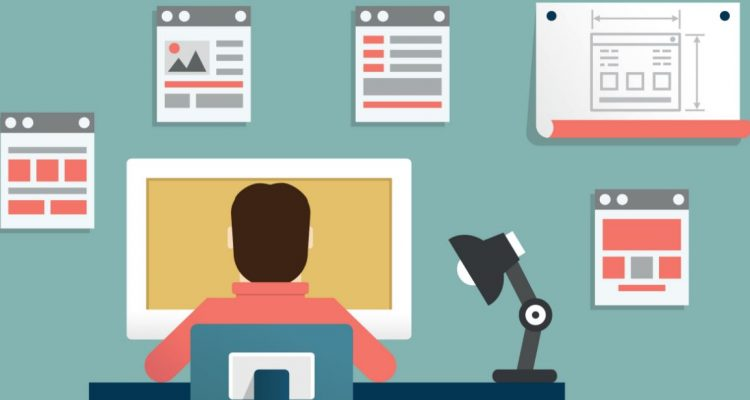
\includegraphics[width=\paperwidth]{Portada2.jpg}};
\draw (current page.center) node [fill=cyan!30!white,fill opacity=0.5,text opacity=1,inner sep=1cm]{\Huge\centering\bfseries\sffamily\parbox[c][][t]{\paperwidth}{\centering GESTIÓN Y MANEJO DEL SISTEMA DE APOYO ALIMENTARIO DE LA UNIVERSIDAD DISTRITAL.\\[15pt] % Book title
{\Large (nombre de la app aun no decidido)}\\[20pt] % Subtitle
{\huge Daniel Garcia Perea 20141020212  \\ Daniel Antonio Moreno Ramirez 20132020620  \\ Edwar Diaz Ruiz 20141020004 \\ Universidad Distrital Francisco José de Caldas}}}; % Author name
\end{tikzpicture}
\vfill
\endgroup

%----------------------------------------------------------------------------------------
%	COPYRIGHT PAGE
%----------------------------------------------------------------------------------------

%\newpage
%~\vfill
%\thispagestyle{empty}

%\noindent Copyright \copyright\ 2017 EconomappGroup\\ % Copyright notice

%\noindent \textsc{Published by Publisher}\\ % Publisher

%\noindent \textsc{book-website.com}\\ % URL

%\noindent Licensed under the Creative Commons Attribution-NonCommercial 3.0 Unported License (the ``License''). You may not use this file except in compliance with the License. You may obtain a copy of the License at \url{http://creativecommons.org/licenses/by-nc/3.0}. Unless required by applicable law or agreed to in writing, software distributed under the License is distributed on an \textsc{``as is'' basis, without warranties or conditions of any kind}, either express or implied. See the License for the specific language governing permissions and limitations under the License.\\ % License information

%\noindent \textit{First printing, Abril 2017} % Printing/edition date

%----------------------------------------------------------------------------------------
%	TABLE OF CONTENTS
%----------------------------------------------------------------------------------------

%\usechapterimagefalse % If you don't want to include a chapter image, use this to toggle images off - it can be enabled later with \usechapterimagetrue

\pagestyle{empty} % No headers
\chapterimage{indice.jpg} % Table of contents heading image
\tableofcontents % Print the table of contents itself
\chapterimage{indice2.jpg} % Table of contents heading image
\listoffigures % indice de figuras
\cleardoublepage % Forces the first chapter to start on an odd page so it's on the right
\pagestyle{fancy} % Print headers again

%%----------------------------------------------------------------------------------------
%%	PARTES
%%----------------------------------------------------------------------------------------
\part{Contextualización}
\chapterimage{problema.jpg} % Table of contents heading image
\chapter{Problema}
\section{Problema}

Dificultad que tienen los estudiantes para aprovechar el apoyo alimentario que ofrece la Universidad Distrital Francisco José de Caldas.



\section{Objetivos}

Crear una aplicación que permita agilizar el proceso de entrega de almuerzo
Mejorar el servicio de apoyo alimentario 
Automatizar el proceso registro de asistencia de usuarios
\\
\\
\textbf{Pregunta: ¿Cómo agilizar el proceso de entrega de almuerzos en la Universidad ?}

\section{Hipotesis:}

Una estrategia para agilizar el proceso de entrega de almuerzos en la universidad es la construcción de un aplicativo web que permita la entrega de papeles, organización de horarios y la verificación de asistencia al apoyo alimentario.
\\
Es necesario que a través del aplicativo se pueda organizar horarios ya que si solo se gestiona la asistencia y entrega de papeles no habra una solucion al problema a largo plazo pero si gestionan los horarios estudiantiles se pueden crear estrategias para evitar el aglutinamiento de personas a la hora de recibir el almuerzo.
\\
\section{Justificación:}
En la Universidad Distrital Francisco José de Caldas existe un serio problema de gestión en la distribución de almuerzo a los estudiante:  la lentitud en la entrega ha ocasionado que los estudiantes no puedan aprovechar el servicio sin correr el riesgo de comprometer la llegada a sus clases. Muchos estudiantes necesitan el apoyo alimentario pero el llegar tarde a clase da lugar incidentes entre profesores y alumnos lo que  puede afectar, a su vez, el desempeño académico
\chapterimage{metodologia.jpg} % Table of contents heading image
\chapter{Metodología}
\section{Manifiesto Agil}
Antes de decir que es Scrum, vale la pena saber que es el manifiesto agil y de que se compone.
\\
\\
El manifiesto agil se compone por 5 valores y 12 Principios:
\\
\\
\subsection{Valores}
\subsubsection{Valorar a las personas y las interacciones entre ellas por sobre los procesos y las herramientas}
Las personas son el principal factor de éxito de un proyecto de software. Es más importante construir un buen equipo que construir el contexto. Muchas veces se comete el error de construir primero el entorno de trabajo y esperar que el equipo se adapte automáticamente. Por el contrario, la agilidad propone crear el equipo y que éste construya su propio entorno y procesos en base a sus necesidades.
\\
\\
\subsubsection{Valorar        el   software       funcionando        por     sobre      la 
	documentación detallada} 
La regla a seguir es "no producir documentos a menos que sean 
necesarios      de    forma     inmediata      para    tomar     un   decisión 
importante". Estos documentos deben ser cortos y centrarse en 
lo esencial. La documentación (diseño, especificación técnica de 
un sistema) no es más que un resultado intermedio y su finalidad 
no    es  dar   valor   en   forma    directa   al   usuario   o   cliente   del 
proyecto. Medir avance en función de resultados intermedios se 
convierte en una simple "ilusión de progreso". 
\\
\\
\subsubsection{Valorar      la   colaboración      con    el   cliente   por    sobre    la 
	negociación de contratos}
Se propone que exista una interacción constante entre el cliente 
y el equipo de desarrollo. Esta mutua colaboración                será la que 
dicte la marcha del proyecto y asegure su éxito. 
\\
\\
\subsubsection{Valorar la respuesta a los cambios por sobre el seguimiento 
	estricto de los planes }
La habilidad de responder a los cambios que puedan surgir a lo 
largo del proyecto (cambios en los requisitos, en la tecnología, 
en el equipo, etc.) determina también su éxito o fracaso. Por lo 
tanto, la planificación no debe ser estricta sino flexible y abierta. 
\\
\\
\subsection{Principios}
Los     valores    anteriores    son    los  pilares    sobre    los  cuales    se 
construyen   los   doce   principios   del   Manifiesto   Ágil.   De   estos 
doce principios, los dos primeros son generales y resumen gran 
parte   del   espíritu   ágil   del   desarrollo   de   software,   mientras   que 
los siguientes son más específicos y orientados al proceso o al 
equipo de desarrollo:\\
\\
\begin{enumerate}[]
	\item   Nuestra mayor prioridad es satisfacer al cliente a través 
	de   entregas     tempranas      y  frecuentes     de   software    con 
	valor.

	\item  Aceptar       el   cambio      incluso     en   etapas     tardías    del 
	desarrollo.   Los   procesos   ágiles   aprovechan   los   cambios 
	para darle al cliente ventajas competitivas.
	\item  Entregar software funcionando en formafrecuente , desde 
	un   par   de   semanas   a   un   par   de   meses,   prefiriendo   el 
	periodo de tiempo más corto.
	\item   Expertos     del   negocio    y  desarrolladores      deben    trabajar 
	juntos diariamente durante la ejecución del proyecto.
	\item   Construir      proyectos     en   torno    a  personas     motivadas, 
	generándoles       el   ambiente      necesario,     atendiendo      sus 
	necesidades y confiando en que ellos van a poder hacer 
	el trabajo.
	\item  La    manera     más    eficiente   y   efectiva    de  compartir      la 
	información       dentro   de   un   equipo    de   desarrollo    es   la 
	conversación cara a cara.
	\item  El   software      funcionando      es   la   principal    métrica    de 
	progreso.
	\item  Los procesos ágiles promueven el desarrollo sostenible. 
	Los     sponsors,    desarrolladores      y  usuarios    deben    poder 
	mantener un ritmo constante indefinidamente.
	\item  La   atención   continua   a   la   excelencia   técnica   y   buenos 
	diseños incrementan la agilidad.
	\item  La   simplicidad    –el    arte  de   maximizar      la  cantidad    de 
	trabajo no hecho- es esencial.
	\item  Las    mejores     arquitecturas,     requerimientos       y   diseños 
	emergen de equipos auto-organizados.
	\item  A   intervalos   regulares,   el   equipo   reflexiona   acerca   de 
	cómo convertirse en más efectivos, luego mejora y ajusta 
	su comportamiento adecuadamente.
\end{enumerate}

\section{Scrum}
Scrum es una de las metodologia agiles mas conocidas al igual que XP, es una herramienta en la cual se tienen varios grupos de trabajo enfocados en diversas tareas con un unico objetivo, en el cual se espera generar resultados y/o entregas al cliente en cortos periodos de tiempo.
\\
\\
El equipo de trabajo en esta metodologia esta apoyado por 2 roles:  El ScrumMaster y el Product Owner. el ScrumMaster o tambien consederado Coach es aquel que vela por que se utilice Scrum , por remover las impedimentos y da asistencia al equipo para que logre el mayor nivel de rendimiento  posible.  El   Product   Owner   es 
quien     representa      al  negocio,  stakeholders ( trabajadores, organizaciones sociales, accionistas y proveedores, entre muchos otros actores clave ),         cliente    y  usuarios 
finales. 
\subsection{En que se basa}

Esta basada en tres pilares:
\\
\\
Transparencia: Todos los implicados tienen conocimiento de qué ocurre y en el proyecto y cómo ocurre. Esto hace que haya un entendimiento “común” del proyecto, una visión global.
\\
\\
Inspección: Los miembros del equipo Scrum frecuentemente inspeccionan el progreso para detectar posibles problemas. La inspección no es un examen diario, sino una forma de saber que el trabajo fluye y que el equipo funciona de manera auto-organizada.
\\
\\
Adaptación: Cuando hay algo que cambiar, el equipo se ajusta para conseguir el objetivo del sprint. Esta es la clave para conseguir éxito en proyectos complejos, donde los requisitos son cambiantes o poco definidos y en donde la adaptación, la innovación, la complejidad y flexibilidad son fundamentales.




\part{Diseño}
\chapterimage{requerimientos.jpg} % Table of contents heading image
\chapter{Requerimientos}
\section{Casos de uso}

El caso de uso es un marco de trabajo que busca hacer representar las acciones que un usuario dado de la aplicación puede hacer en ella, pero no en términos computacionales, en donde el desarrollador crea las funciones de la capa lógica y de persistencia, sino en un sentido mas natural para el, siendo esto los subproblemas derivados del problema principal.

Los casos de uso se crean para refinar un conjunto de requisitos de acuerdo con una función o tarea. En lugar de la tradicional lista de requisitos que quizá no trate de forma directa el uso de la solución, los casos de uso reúnen requisitos comunes basados en el tipo de función u objetivo. Los casos de uso definen qué harán los usuarios o funciones en la solución y un proceso empresarial define cómo realizarán esas funciones \cite{Pw2CU}.

Para el diseño de casos de uso se debe seguir la siguiente nomenclatura:
\begin{itemize}
	\item El usuario que va a usar la aplicación es una figura humanioide y debajo de este esta descrito el rol, que es su papel en el programa
	\item Cada acción del usuario se representa con un circulo y dentro se agrega una breve descripción de la funcionalidad.
	\item Para relacionar a un usuario con una acción en particular se usa una linea sin direcciones si la interacción es bidireccional, o con dirección de acuerdo a orientación de la operación
	\item Para relacionar dos casos de uso, es mediante una flecha segmentada, en donde hay dos tipos de relaciones principales:
	\begin{itemize}
		\item  \textbf{include:} Representa una relación de dependencia, en donde el caso de uso origen necesita del caso de uso de llegada.
		\item \textbf{extend:} Describe una relación de necesidad opcional, en donde el caso de uso del que parte puede es opcional del caso de uso al que llega.
	\end{itemize}
\end{itemize}

A en la figura 3.1 se puede visualizar el caso de uso destinado a este software, allí, se describe lo qué debe hacer el programa.

\begin{figure}[H]
	\centering
	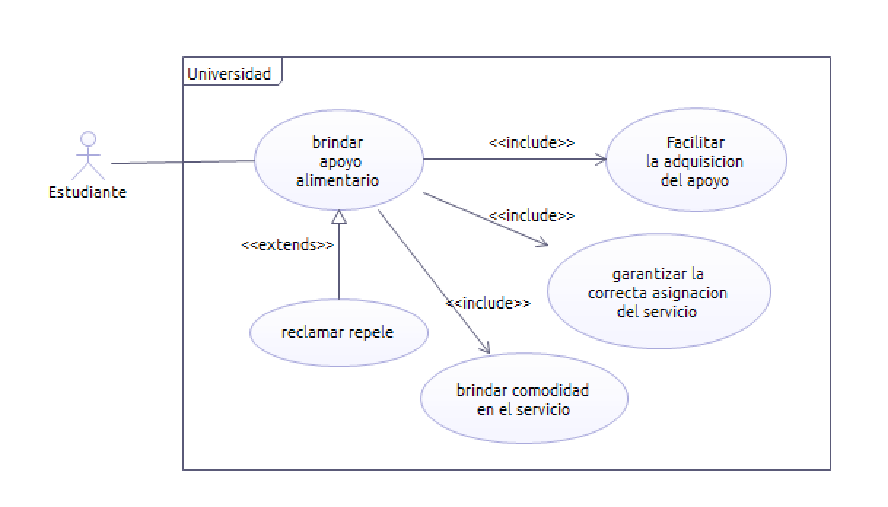
\includegraphics[width=0.8\linewidth]{parte2/imgs/CasosDeUso/caso1}
	\caption{Diagrama de caso de uso}
	\label{fig:diagramadecasodeuso}
\end{figure}

\section{Requerimientos de Casos de uso}

Los requerimientos de caso de uso entregan el plan de interacción entre el usuario y cada caso de uso: la descripción del caso de uso, los pasos para realizarse, las posibles fallas a las que puede incurrir, la prioridad y urgencia y comentarios acerca del mismo, todo para delimitar correctamente la relación usuario-aplicación
\begin{table}[H]
	\centering
	\caption{Caso de Uso CU-1}
	\label{my-label1}
	\begin{tabular}{|l|l|}
		\hline
		\textbf{Nombre}      & Brindar Apoyo Alimentario                                                                                                                                                   \\ \hline
		\textbf{Actores}     & Estudiantes                                                                                                                                                                 \\ \hline
		\textbf{Escenario}   &                                                                                                                                                                             \\ \hline
		\textbf{Primario}    & Brindar Apoyo Alimentario                                                                                                                                                   \\ \hline
		\textbf{Secundario}  & No coinciden Horarios                                                                                                                                                       \\ \hline
		\textbf{Excepciones} & \begin{tabular}[c]{@{}l@{}}Solicitud de Inscripción no aceptada, Estudiante no Registrado,\\ Se acabo el alimento, Ser retirado del beneficio por alguna falla\end{tabular} \\ \hline
	\end{tabular}
\end{table}

\begin{table}[H]
	\centering
	\caption{Caso de Uso CU-2}
	\label{my-label2}
	\begin{tabular}{|l|l|}
		\hline
		\textbf{Nombre}      & Reclamar Repele                                                                                                                                          \\ \hline
		\textbf{Actores}     & Estudiantes                                                                                                                                              \\ \hline
		\textbf{Escenario}   &                                                                                                                                                          \\ \hline
		\textbf{Primario}    & Reclamar Repele                                                                                                                                          \\ \hline
		\textbf{Secundario}  &                                                                                                                                                          \\ \hline
		\textbf{Excepciones} & \begin{tabular}[c]{@{}l@{}}No sobro alimento, Estudiante no Registrado, Ser retirado del beneficio,\\ La hora del reclamo no es la adecuada\end{tabular} \\ \hline
	\end{tabular}
\end{table}

\begin{table}[H]
	\centering
	\caption{Caso de Uso CU-3}
	\label{my-label3}
	\begin{tabular}{|l|l|}
		\hline
		\textbf{Nombre}      & Brindar Comodidad en el Servicio                                                                                                                                            \\ \hline
		\textbf{Actores}     & Administrativos, Estudiantes                                                                                                                                                \\ \hline
		\textbf{Escenario}   &                                                                                                                                                                             \\ \hline
		\textbf{Primario}    & Brindar Comodidad en el Servicio                                                                                                                                            \\ \hline
		\textbf{Secundario}  & Presentar Inscripción en la fechas no estipuladas                                                                                                                           \\ \hline
		\textbf{Excepciones} & \begin{tabular}[c]{@{}l@{}}Se presenta algún error en la Infreestructura, No se abríran convocatorias\\ No se cuentan con los espacios o horarios disponibles.\end{tabular} \\ \hline
	\end{tabular}
\end{table}

\begin{table}[H]
	\centering
	\caption{Casso de Uso CU-4}
	\label{my-label4}
	\begin{tabular}{|l|l|}
		\hline
		\textbf{Nombre}      & Garantizar Correcta Asignación del Servicio                                                                                                                                                                                       \\ \hline
		\textbf{Actores}     & Empleados y Administrativos encargados del apoyo                                                                                                                                                                                  \\ \hline
		\textbf{Escenario}   &                                                                                                                                                                                                                                   \\ \hline
		\textbf{Primario}    & Garantizar Correcta Asignación del Servicio                                                                                                                                                                                       \\ \hline
		\textbf{Secundario}  & \begin{tabular}[c]{@{}l@{}}Presentarse en las horas no adecuadas, Presentar alguna inconveniente\\ en un requerimiento del Apoyo\end{tabular}                                                                                     \\ \hline
		\textbf{Excepciones} & \begin{tabular}[c]{@{}l@{}}Fallos en la Infreestructura, Falla del Personal encargado de brindar\\ el servicio, Inconvenientes presentados tanto en espacios como\\ horarios habilitados para la entrega del servicio\end{tabular} \\ \hline
	\end{tabular}
\end{table}

\begin{table}[H]
	\centering
	\caption{Caso de Uso CU-5}
	\label{my-label5}
	\begin{tabular}{|l|l|}
		\hline
		\textbf{Nombre}      & Facilitar Adquisición del Apoyo                                                                                                                                                      \\ \hline
		\textbf{Actores}     & Administrativos, Personal encargado de brindar el servicio                                                                                                                           \\ \hline
		\textbf{Escenario}   &                                                                                                                                                                                      \\ \hline
		\textbf{Primario}    & Facilitar Adquisión del Apoyo                                                                                                                                                        \\ \hline
		\textbf{Secundario}  & Presentar alguna inconsistencia en la inscripción o documentos que soportan la misma,                                                                                                \\ \hline
		\textbf{Excepciones} & \begin{tabular}[c]{@{}l@{}}Fallos en la Infreestructura, No poder optar por el beneficio por falta de cupos,\\ No tener el puntaje necesarios para recibir el beneficio\end{tabular} \\ \hline
	\end{tabular}
\end{table}

\clearpage
% Please add the following required packages to your document preamble:
% \usepackage[table,xcdraw]{xcolor}
% If you use beamer only pass "xcolor=table" option, i.e. \documentclass[xcolor=table]{beamer}

%requerimientos, casos de uso
\chapterimage{analisis.jpg} % Table of contents heading image
\chapter{Análisis del sistema e interacción}

La interacción del sistema se puede visualizar mediante diagramas de secuencia, con los cuales se podrá hacer un análisis más clarificado sobre cómo es el ciclo de vida del programa y de qué forma son las relaciones internas de éste.

Para detallar un poco más sobre la comunicación de las partes del sistema, es indispensable un diagrama de comunicación, en donde se podrá detallar los que se transmite entre los objetos, es similar al diagrama de secuencia pero no describe un orden de transmisión de mensajes sino que se centra en los mismos mensajes dados.

Por ultimo, para aclarar cómo se compone el sistema, se explicarán los diagramas de clases, éstos describen cómo están conformadas las calases del sistema, cómo son sus relaciones y sobretodo, cuales son los patrones de diseño que se implementan en la aplicación y cómo optimizan el  funcionamiento de la misma.

%%%%%%%%%%%%%%%%%%%%%% Sección 4.1 %%%%%%%%%%%%%%%%%%%%%%%%%%%
\section{Diagramas de secuencia}

Un diagrama de secuencia muestra una interacción, que representa la secuencia de mensajes entre instancias de clases, componentes, subsistemas o actores. El tiempo fluye por el diagrama y muestra el flujo de control de un participante a otro. Utilice diagramas de secuencia para visualizar instancias y eventos, en lugar de clases y métodos. En el diagrama, puede aparecer más de una instancia del mismo tipo. También puede haber más de una ocurrencia del mismo mensaje \cite{Pw3DS}.

Un diagrama de secuencia es aquel en el que se muestra la interacción entre actores, objetos, interfaces, controles, bases de datos y otras entidades a través del tiempo según el enfoque, el cual puede ser:
\begin{itemize}
	\item \textbf{Enfoque de objetos}: donde son participes las relaciones que existen entre éstos y con actores para realizar una tarea determinada.
	\item \textbf{Enfoque de modelado a tres capas}: donde el actor se comunica con una entidad interfaz, y ésta a su vez con una entidad control para llegar a una persistencia. 
\end{itemize}

Es importante resaltar que cada diagrama de secuencia se realiza en torno a la descripción de un caso de uso dado, ya que éste define el orden en que se deban distribuir las tareas para cada una de las entidades que son participes a la hora de representar cada caso.

Para este proyecto se realizaron 5 casos de uso de los cuales se va a crear un diagrama de secuencia por cada caso y uno para cada enfoque. Inicialmente el caso de uso de .

A continuación se describirá cada diagrama de secuencia:

\paragraph{Diagrama del control de asistencia}

\begin{figure}[H]
	\centering
	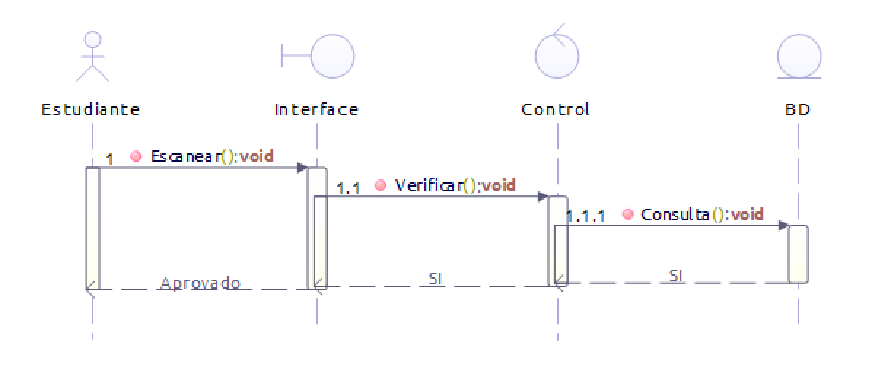
\includegraphics[width=1\linewidth]{parte2/imgs/DiagramaSecuencia/Asistencia}
	\caption[Diagrama de secuencia de registro de Asistencia]{Diagrama de secuencia para el registro del control de asistencia}
	\label{fig:diagramadesecuencia1}
\end{figure}
Este diagrama de secuencia explica el funcionamiento del programa frente al control de asistencia de los estudiantes al apoyo alimentario.
\\
Para este caso el estudiante representa el usuario que ingresa al programa y que mediante el escaneo del codigo del carnet realiza la actualizacion de asistencia en la base de datos.

 





\paragraph{Diagrama del Registro de usuarios}
\begin{figure}[H]
	\centering
	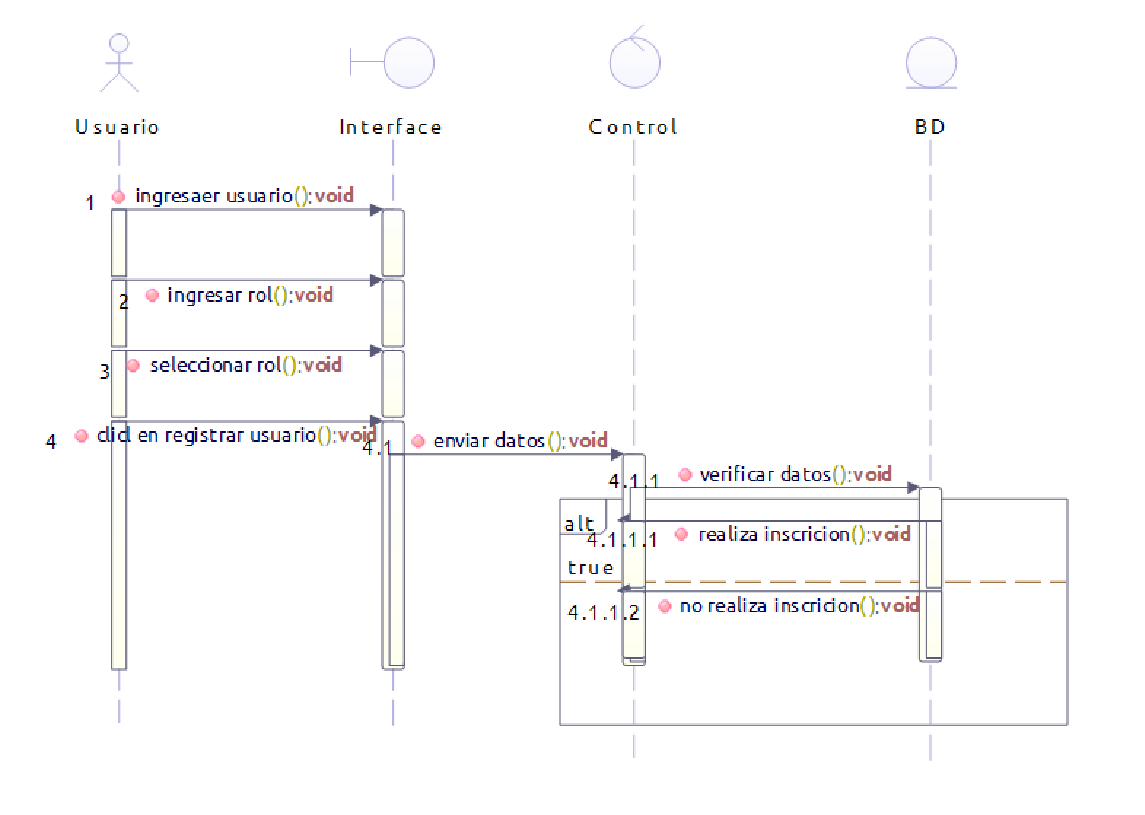
\includegraphics[width=0.8\linewidth]{parte2/imgs/DiagramaSecuencia/RegUsu}
	\caption[Diagrama de secuencia Registrar Usuario]{Diagrama de secuencia para el registro de usuarios}
	\label{fig:diagramadesecuencia2}
\end{figure}

Este diagrama de secuencia representa el registro de un usuario. Para lo cual el usuario ingresa sus datos selecciona un rol y realiza el click para registrar los datos y consulta dentro de la base de datos la existencia del usuario y si existe se envia un mensaje que alerta sobre la existencia del usuario. 



\paragraph{Diagrama para crear nuevas convocatorias}
\begin{figure}[H]
	\centering
	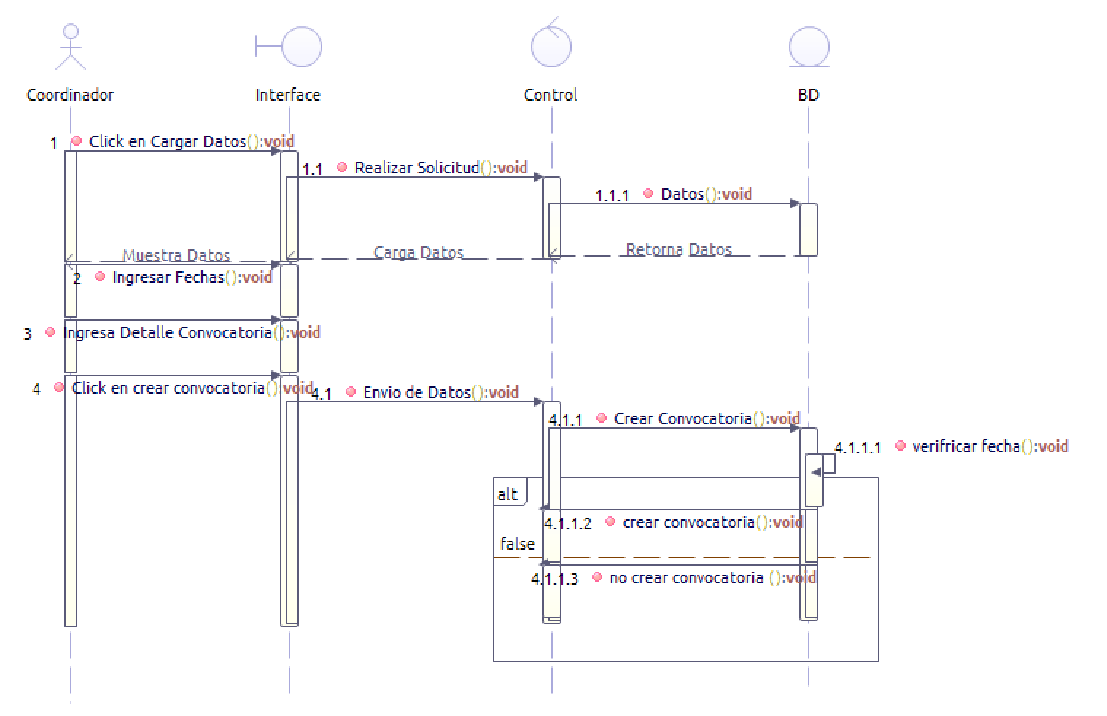
\includegraphics[width=0.8\linewidth]{parte2/imgs/DiagramaSecuencia/SecCrearConv}
	\caption[Diagrama de secuencia Crear convocatoria]{Diagrama de secuencia para crear una nueva convocatoria}
	\label{fig:diagramadesecuencia5}
\end{figure}
Este diagrama de secuencia representa el registro de convocatorias de apoyo alimentario dentro del aplicativo.El programa registra los datos para los cuales nescesita realizar la carga  datos, fechas y detalles especificos de cada convocatoria que al final mediante una consulta a la base de datos define si se puede crear o no la convocatoria.


 
\paragraph{Diagrama del registro a convocatoria existentes}
\begin{figure}[H]
	\centering
	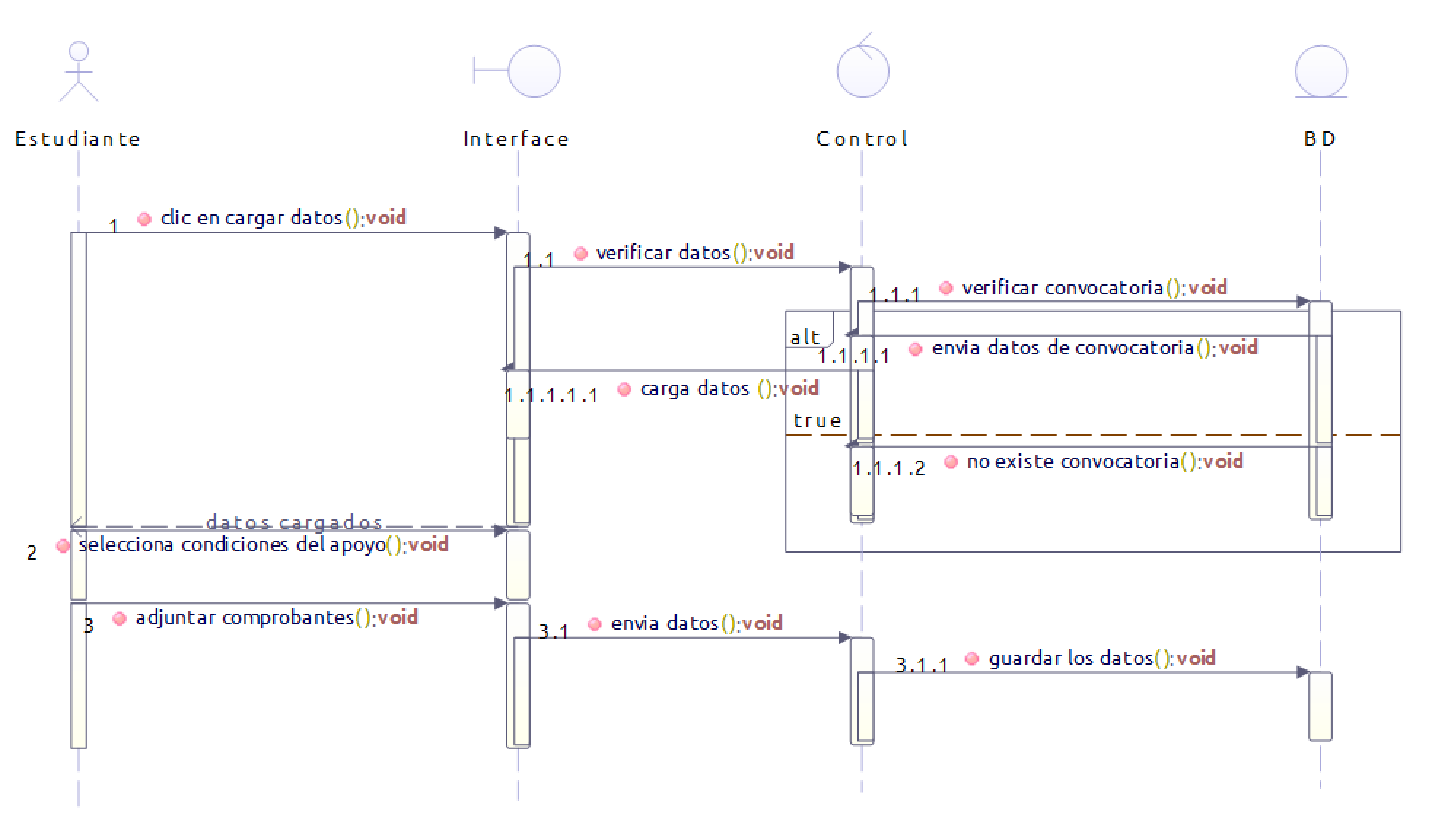
\includegraphics[width=0.8\linewidth]{parte2/imgs/DiagramaSecuencia/SecSolConv}
	\caption[Diagrama de secuencia Registro a una convocatoria]{Diagrama de secuencia para el registro a una convocatoria}
	\label{fig:diagramadesecuencia3}
\end{figure}

En este diagrama se realiza la solicitud de los usuarios a una nueva convocatoria. Para este proceso es nescesario que los usuarios carguen toda la informacion que luego se registra en la base de datos.


\paragraph{Diagrama de la verificacion de una solicitud a una convocatoria}
\begin{figure}[H]
	\centering
	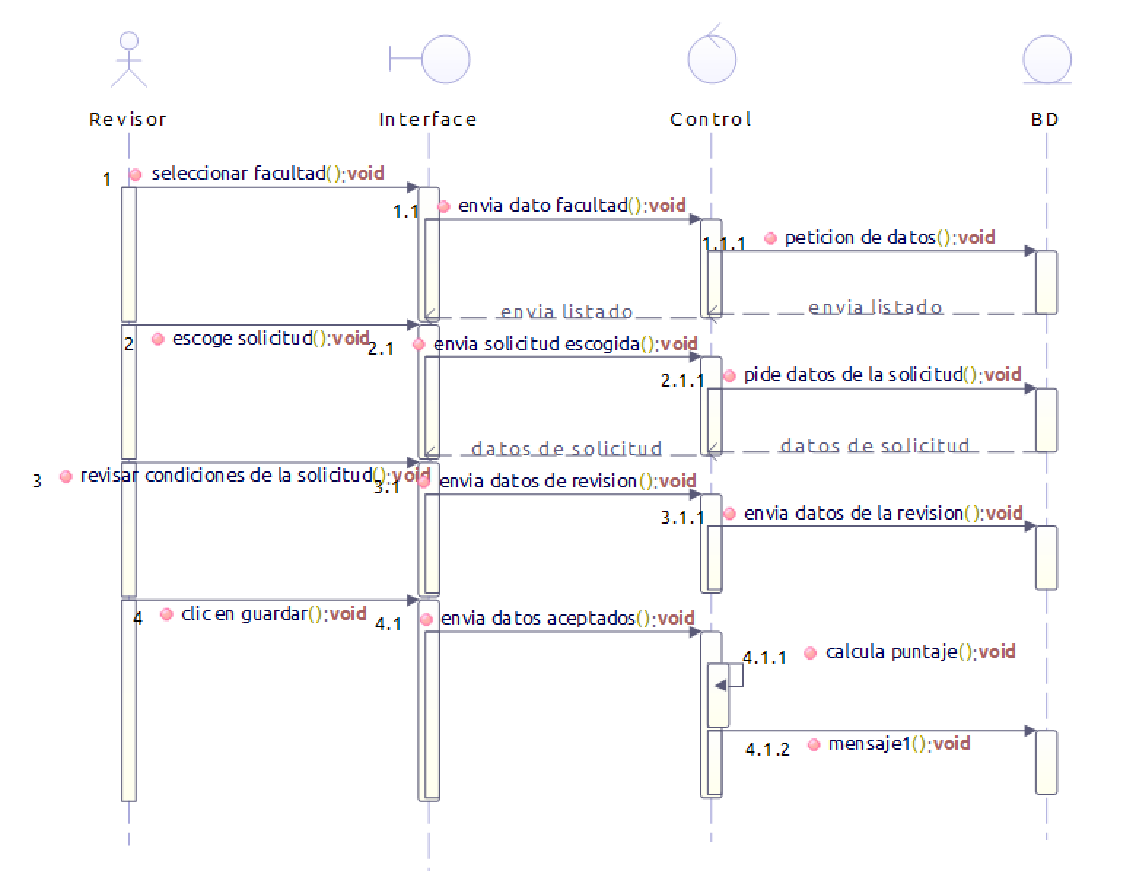
\includegraphics[width=0.8\linewidth]{parte2/imgs/DiagramaSecuencia/SecVerifSolConv}
	\caption[Diagrama de secuencia Verificacion de solicitud]{Diagrama de secuencia de verificacion de una solicitud a una convocatoria}
	\label{fig:diagramadesecuencia4}
\end{figure}

Para este diagrama representamos la intereaccion que tiene un usuario revisor con las solicitudes presentes en la base de datos. En este caso el revisor realiza la seleccion de la facultad y se muestra un listado de las solicitudes de dicha facultad y se escoge la solicitud y consulta en la base de datos la solicitud escogida. Envia los datos de la revision y los datos aceptados a los cuales le calcula el puntaje y envia los datos a la base de datos

\newpage

%%%%%%%%%%%%%%%%%%%%%% Sección 4.2 %%%%%%%%%%%%%%%%%%%%%%%%%%%
\section{Diagramas de comunicación}

También llamados Diagramas de Colaboración. Nos sirven para enfatizar los vínculos de datos entre los participantes de una interacción. Un diagrama de Comunicación modela las interacciones entre objetos o partes en términos de mensajes en secuencia. Los diagramas de Comunicación representan una combinación de información tomada desde el diagrama de Clases, Secuencia, y Diagrama de casos de uso describiendo tanto la estructura estática como el comportamiento dinámico de un sistema \cite{Pw4DC}.

Los diagramas de comunicación tienen la función de simplificar la visualización de los modelos, dado que se enfocan exclusivamente en los objetos y su interacción, la cual se hace por medio de mensajes. Para seguir la lectura de un diagrama de comunicación se procede a ubicar el mensaje con la enumeración de primer orden, y se sigue la dirección indicada por la flecha adjunta, y así sucesivamente hasta llegar al último mensaje. Este tipo de diagrama se encuentra muy relacionado con el diagrama de secuencia, dado un isomorfismo entre éstos; Son equivalentes, pero tienen dos puntos de vista.


\paragraph{Diagrama del control de asistencia}
\begin{figure}[H]
	\centering
	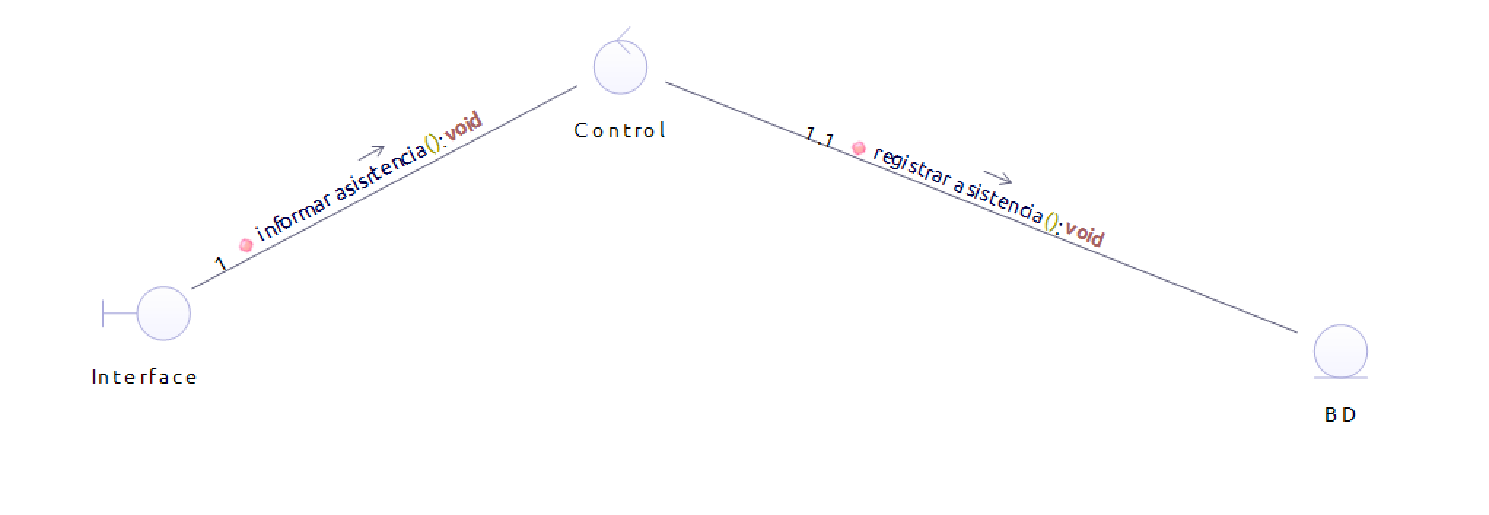
\includegraphics[width=1\linewidth]{parte2/imgs/DiagramaComunicacion/ComAsist}
	\caption[Diagrama de Comunicacion Control de asistencia]{Diagrama de Comunicación del control de asistencia}
	\label{fig:diagramaDeComunicacion}
\end{figure}

En la figura 4.6 la interfaz envia el mensaje "informar asistencia()" al objeto control que a su vez envia un mensaje "regisrarasistencia()" a la base de datos.


\newpage
%newpage para machetear y que no se vea tan paila

\paragraph{Diagrama del registro de usuarios}
\begin{figure}[H]
	\centering
	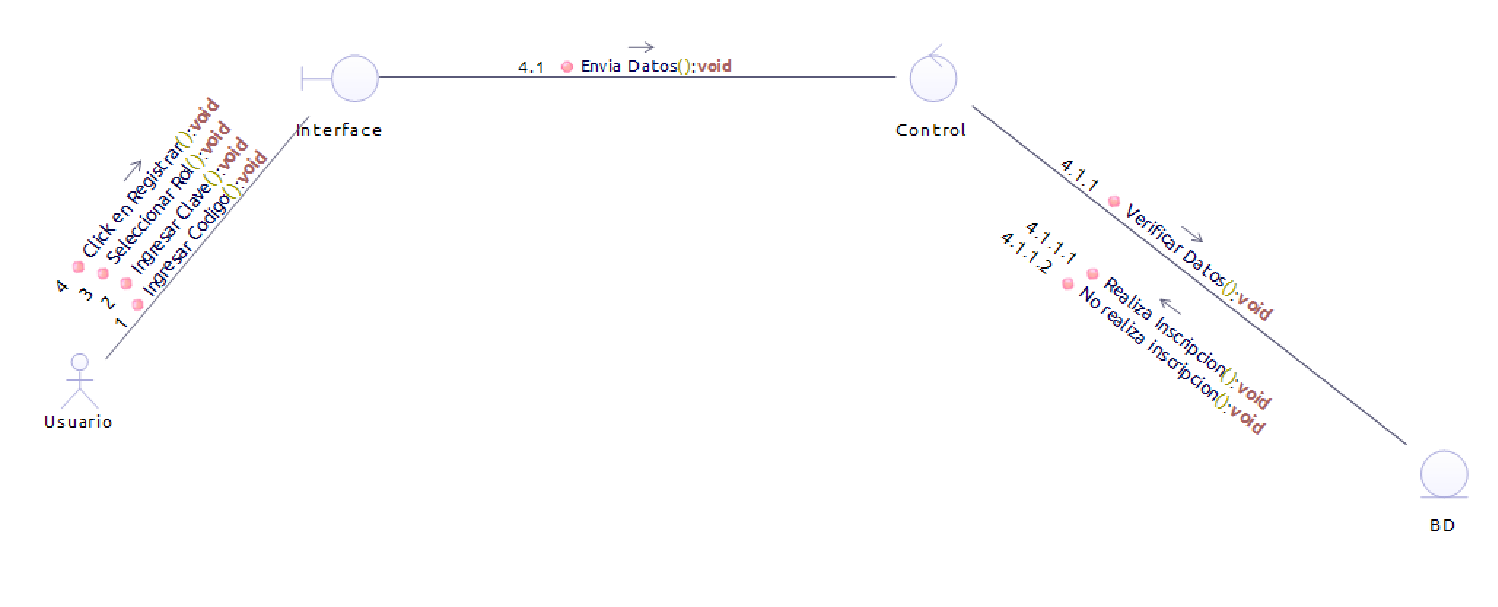
\includegraphics[width=1\linewidth]{parte2/imgs/DiagramaComunicacion/ComReguU}
	\caption[Diagrama de Comunicacion del registro de usuarios]{Diagrama de Comunicación del registro de usuarios}
	\label{fig:diagramaDeComunicacion3}
\end{figure}

En la figura 4.7 el usuario envia los mensajes "IngresarClave()", "IngrearCodigo()" a la interface,la interface envia el siguiente mensaje "EnviarDatos()"  al control 

\paragraph{Diagrama de la creacion de una convocatoria}
\begin{figure}[H]
	\centering
	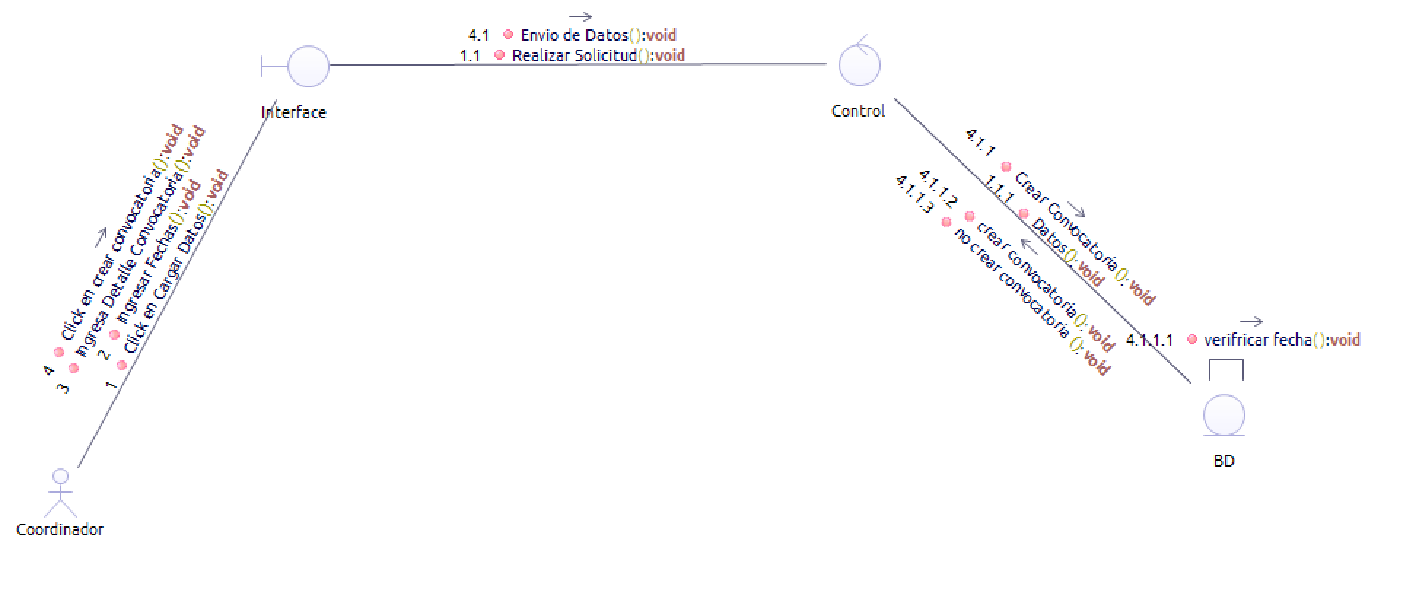
\includegraphics[width=1\linewidth]{parte2/imgs/DiagramaComunicacion/ComCreConv}
	\caption[Diagrama de Comunicacion cfracion Covoactoria]{Diagrama de Comunicación de la creacion de una convocatoria}
	\label{fig:diagramaDeComunicacion5}
\end{figure}

En la figura 4.8 el coordinador  envia los datos a la interfaz mediante el mensaje "cargarDatos()" y la interface mediante "EnvioDatos()" envia los datos a la base de datos y mediante "RealizarSolicitud()" envia datos de la solicitud a la base de datos, la base de datos recive "datos()" y se envia un mensaje de verificacion de datos "verificarfecha()".

\paragraph{Diagrama para la solicitud a una convocatoria}
\begin{figure}[H]
	\centering
	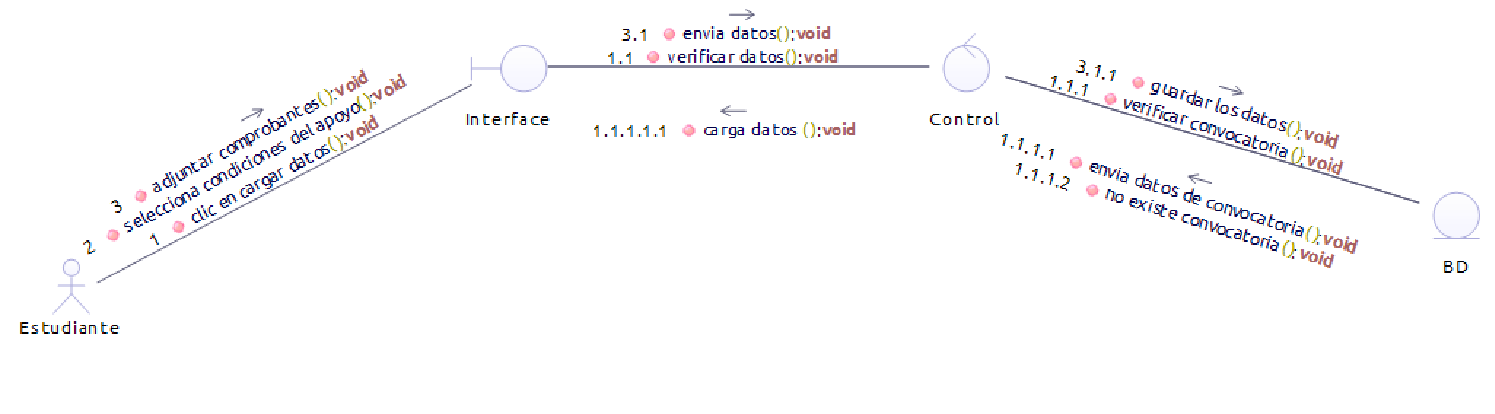
\includegraphics[width=1\linewidth]{parte2/imgs/DiagramaComunicacion/ComSoliConv}
	\caption[Diagrama de Comunicacion Solicitud a Convocatoria]{Diagrama de Comunicación para la solicitud a una convocatoria}
	\label{fig:diagramaDeComunicacion2}
\end{figure}

Para la figura 4.9  el estudiante envia los datos para la solicitud de la convocatoria a la interfaz y la interfaz envia y recive mensaje a la base de datos

\paragraph{Diagrama de la verificacion de una solicitud}
\begin{figure}[H]
	\centering
	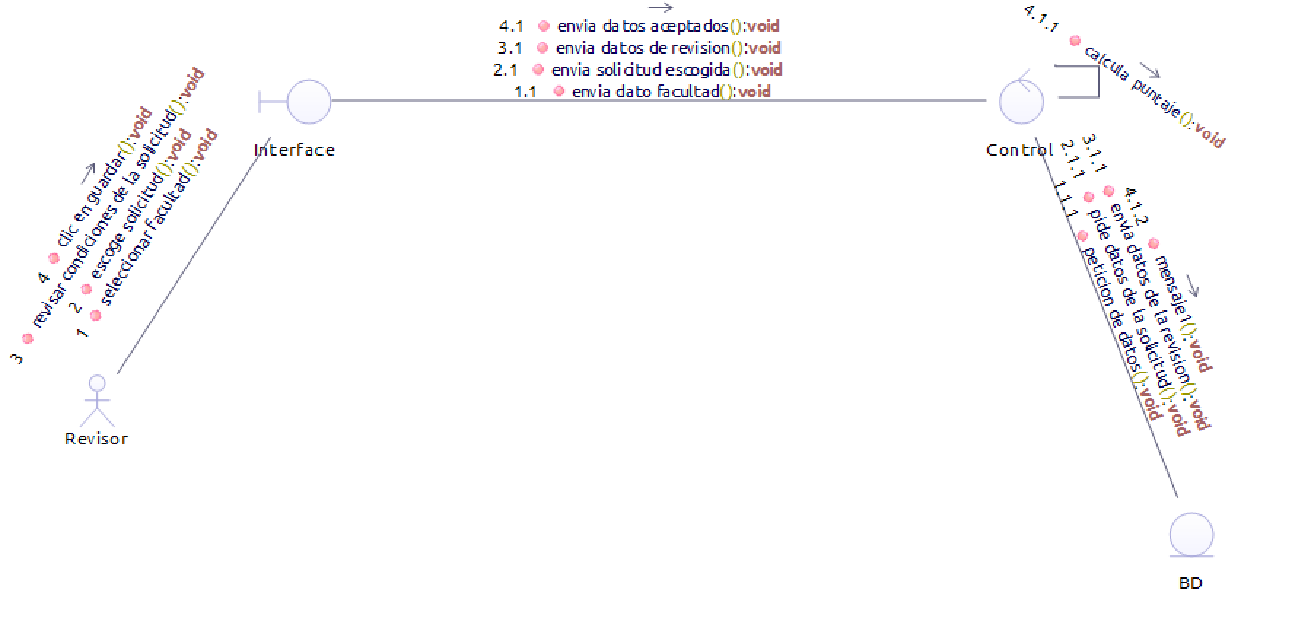
\includegraphics[width=1\linewidth]{parte2/imgs/DiagramaComunicacion/ComVer}
	\caption[Diagrama de Comunicacion verificacion solicitud]{Diagrama de Comunicación de la  verificacion de una solicitud}
	\label{fig:diagramaDeComunicacion4}
\end{figure}

Para figura 4.10 el revisor realiza las peticiones de las solicitudes mediante la interfaz a la base de datos y revisa los datos de los solicitantes para que despues se calcule el puntaje 

\newpage

%%%%%%%%%%%%%%%%%%%%%% Sección 4.3 %%%%%%%%%%%%%%%%%%%%%%%%%%%
\section{Diagramas de clases}

Para una análisis orientado al desarrollo del aplicativo se plantean los diagramas de clases, que básicamente representa la interacción entre distintas entidades que en conjunto logran cumplir con la funcionalidad del programa. Los diagramas de clases se componen principalmente de:

\begin{itemize}
	\item  \textbf{Clase}: Esta es la entidad que representara un objeto que interviene en la solución del problema. Su ilustración es un rectángulo dividido en 3 niveles: En el primero esta el nombre, el segundo es para los atributos y el ultimo es para las operaciones de dicho objeto
	\item \textbf{Relación}: Las relaciones se encargan de mostrar como es la interacción entre las clases de un diagrama, permite la comunicación entre las mismas y se dividen en 4 fundamentalmente
	
	
	\begin{itemize}
		\item \textit{\textbf{Herencia}}: Se encuentra en las clases cuando una clase "es una" clase aparte ya definida, en donde la herencia permite realizar una especialización, o en sentido inverso, hacer una generalización de unas características o comportamientos.
		\item \textit{\textbf{Dependencia}}: Se da cuando una clase depende de otra para su existencia o uso, pero la existencia de la primera no interfiere en la existencia de la segunda.
		\item \textit{\textbf{Asociación}}: Ocurre cuando una clase puede usar otra sin que sea obligatorio inicializarla al iniciar la clase principal
		\item \textit{\textbf{Composición}}: Es parecida a la asociación, sin embargo, esta relación hace obligatoria la inicialización de la clase agregada al momento de usar la clase principal.
	\end{itemize}
\end{itemize}

Haciendo uso de las clases y relaciones en un diagrama se puede llegar a una solución para el problema en un momento especifico en el tiempo, pero hay que tener en cuenta que el software debe poder perdurar en el tiempo de forma limpia, sin necesidad de hacer cambios como tal en el código existente sino solo permitir la adición de componentes o clases, para ello se usan los patrones de diseño que no son mas sino estructuras de clases y relaciones enfocadas solucionar los problemas del mantenimiento del software, mejorando así el ciclo de vida de la aplicación.

En los siguientes diagramas se mostraran algunos patrones de diseño en nuestra aplicación enfocados a distintos problemas al momento de plasmar la aplicación en un diagrama de clases.

\subsection{Creacionales}

\paragraph{Builder}
\begin{figure}[H]
	\centering
	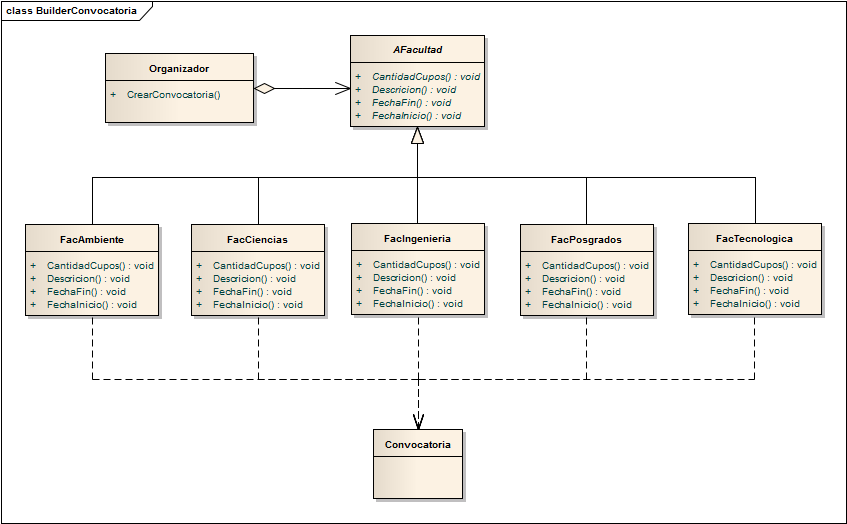
\includegraphics[width=1\linewidth]{parte2/imgs/Patrones/BuilderConvocatoria}
	\caption[Diagrama de clases del patrón Builder]{Diagrama de Clase para creación de de convocatorias por facultad}
	\label{fig:fabricaAbstracta}
\end{figure}

Como Patrón de diseño, el patrón builder (Constructor) es usado para permitir la creación de una variedad de objetos complejos desde un objeto fuente (Producto), el objeto fuente se compone de una variedad de partes que contribuyen individualmente a la creación de cada objeto complejo a través de un conjunto de llamadas a interfaces comunes de la clase Abstract Builder. En este caso la construccion se hace a travez de la creacion de convocatorias de cada facultad.


\paragraph{Factory}
\begin{figure}[H]
	\centering
	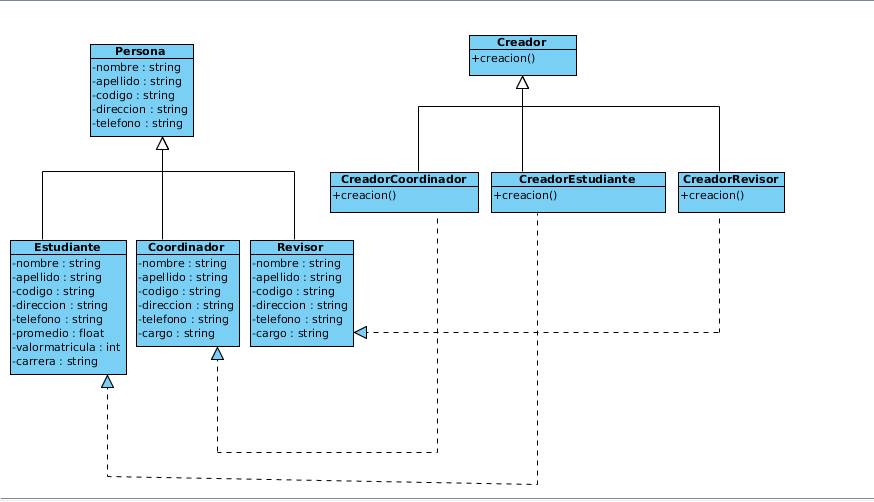
\includegraphics[width=1\linewidth]{parte2/imgs/Patrones/FactoryMethod}
	\caption[Diagrama de clases del patrón Facade]{Diagrama de Clase para el manejo de la conexión a distintas bases de datos a través del patrón de diseño Facade}
	\label{fig:facade}
\end{figure}

En diseño de software, el patrón de diseño Factory Method consiste en utilizar una clase constructora (al estilo del Abstract Factory) abstracta con unos cuantos métodos definidos y otro(s) abstracto(s): el dedicado a la construcción de objetos de un subtipo de un tipo determinado. Es una simplificación del Abstract Factory, en la que la clase abstracta tiene métodos concretos que usan algunos de los abstractos; según usemos una u otra hija de esta clase abstracta, tendremos uno u otro comportamiento. En esta caso implementamos el patron Factory Method para la creacion de diferentes personas que pueden ser estudiantes,coordinador y revisor ya que a pesar de ser hijos del mismo tipo las clases realizan distintas funciones en el software. 

\paragraph{Singleton}
\begin{figure}[H]
	\centering
	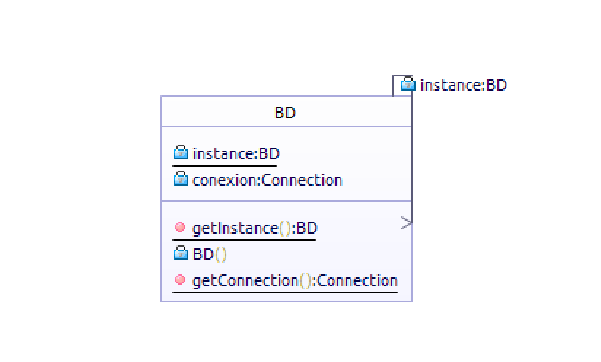
\includegraphics[width=1\linewidth]{parte2/imgs/Patrones/Singleton}
	\caption[Diagrama de clases del patrón Singleton]{Diagrama de Clase para el manejo de las operaciones de escritura/lectura sobre base de datos a través del patrón de diseño Bridge}
	\label{fig:puente}
\end{figure}

En ingeniería de software, singleton o instancia única es un patrón de diseño que permite restringir la creación de objetos pertenecientes a una clase o el valor de un tipo a un único objeto. Su intención consiste en garantizar que una clase sólo tenga una instancia y proporcionar un punto de acceso global a ella.El patrón singleton se implementa creando en nuestra clase un método que crea una instancia del objeto sólo si todavía no existe alguna. Para asegurar que la clase no puede ser instanciada nuevamente se regula el alcance del constructor (con modificadores de acceso como protegido o privado). En este caso aplicamos este patron para controlar el acceso a la base de datos.

\subsection{Comportamiento}

\paragraph{Iterador}
\begin{figure}[H]
	\centering
	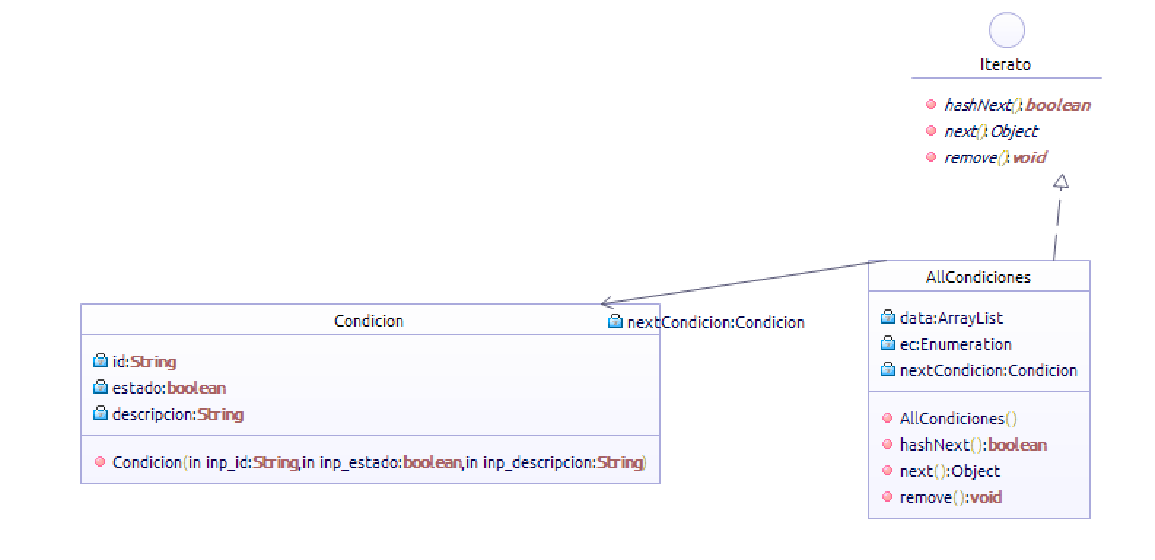
\includegraphics[width=1\linewidth]{parte2/imgs/Patrones/Iterador}
	\caption[Diagrama de clases del patrón Iterador]{Diagrama de Clase para la ejecucion de acciones de CRUD mediante el patron de diseño Comando}
	\label{fig:command}
\end{figure}

Proporcionar una forma de acceder a los elementos de un objeto agregado de forma secuencial sin exponer sus detalles. En este caso me permite analizar todas las condiciones que hay para evaluar el puntaje de la solicitud al apoyo alimentario.



\paragraph{State}
\begin{figure}[H]
	\centering
	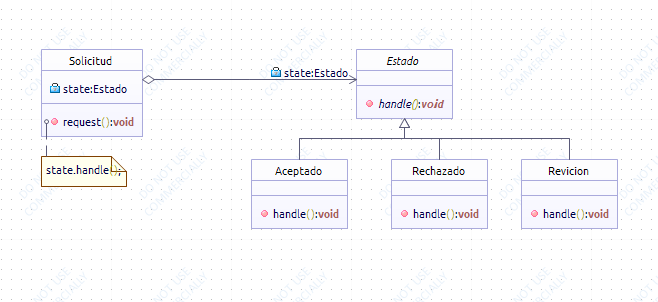
\includegraphics[width=1\linewidth]{parte2/imgs/Patrones/Estado}
	\caption[Diagrama de clases del patrón State]{Diagrama de Clase para la relacion entre flujos financieros y sugerencias mediante el patron de diseño Mediator}
	\label{fig:mediador}
\end{figure}
El patrón de diseño State se utiliza cuando el comportamiento de un objeto cambia dependiendo del estado del mismo. Por ejemplo: una alarma puede tener diferentes estados, como desactivada, activada, en configuración. En este caso permite manejar el estado el cambio de una solicitud de aceptado, rechazado y revicion.

%secuencia,comunicacion, patrones
%\chapterimage{estados.jpg} % Table of contents heading image
\chapter{Estados}

Un estado es una situación durante la vida de un objeto, de forma que cuando dicha situación se satisface se lleva a cabo alguna acción o se espera por un evento. El estado de un objeto se puede caracterizar por el valor de una o varias de las características de su clase, además, el estado de un objeto también se puede caracterizar por la existencia de un enlace con otro objeto. El diagrama de estados y transiciones incluye todos los mensajes que un objeto puede enviar o recibir. En un diagrama de estados, un escenario simboliza un camino dentro del diagrama. Dado que generalmente el espacio entre dos envíos de mensajes representa un estado, se pueden utilizar los diagramas de secuencia para buscar los diferentes estados de un objeto \cite{Pw5DE}.

Nuestro software posee elementos que tiene diferentes estados, para poder observar como estos estados cambian, y cuales son las condiciones de transición entre estos, de mostrará a continuación un diagrama de estados donde se resume todo esto.

\section{Diagrama de Estados}

Los diagramas de estado son un método conocido para explicar el comportamiento de un sistema. Que explican todos los estados posibles en los que puede ingresar un objeto particular y la manera en que modifica el estado del objeto, como resultado de los eventos que llegan a el. Permite identificar bajo qué pruebas se ejecuta cada uno de los procesos y en qué momento podrían tener una variación. El diagrama de estados permite visualizar de una forma ordenada la ejecución de cada uno de los procesos \cite{Pw5DE}.

La siguiente figura muestra el ciclo de vida que puede tener una solicutud a la adquisicion al apoyo alimentario el cual puede encontrarse en tres diferentes estados, REVISION, ACEPTADO,RECHAZADO. Aquel evento odetonador que provoca el cambio de estado es las Condiciones el cual envia un True o unFalse dependiendo de como lo evalue el revisor y determine si dicha solicitusd cumple los requisitos. Ahora bien, existen dos transiciones entre cada fase:
\bigskip
\begin{itemize}
	\item De estado REVISION a ACEPTADO:este cambio de estado se provoca cuando la evaluacion del revisor determina que la solicitud cumple las condiciones y da su visto bueno a dicha solicitud, asignadole al detonador Condiciones el valor de True produciendo el cambio de estado.
	
	\item De estado REVISION a RECHAZADO: es cambio entre estos estados es producido cuando el revisor determina que la solicitud enviada no cumple con las condiciones necesrias para adquirir el beneficio ya sea por falta de datos o por datos incorrectos, en dicho caso el revisor rechaza la solicitud ,asignado al detonador condiciones el valor de False, provocando el cambio de estado.
	
\end{itemize}

\begin{figure}[H]
	\centering
	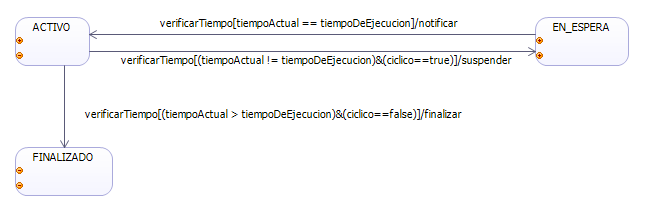
\includegraphics[width=1\linewidth]{parte2/imgs/DiagramaDeEstado/Estados}
	\caption{Diagrama de Estado}
	\label{fig:diagramaEstado}
\end{figure}

\paragraph{Diagrama de clases} 

En el siguiente esquema se muestra la clase foco que es GestionSolicitud, ésta es la que cambia de estados según las condiciones dadas, para ello debe tener como atributos un ESTADO, que es el que va a variar, y los métodos necesarios para actuar a la hora de cambiar de estado.

\begin{figure}[H]
	\centering
	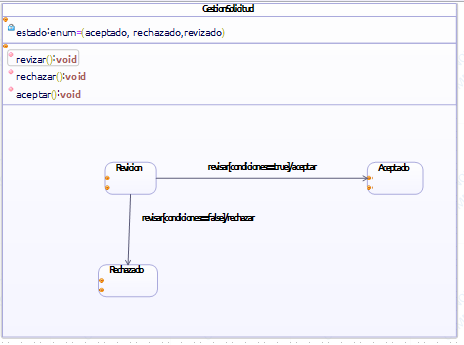
\includegraphics[width=0.8\linewidth]{parte2/imgs/DiagramaDeEstado/claseEstados}
	\caption{Diagrama de Clase Gestion de Solicitud}
	\label{fig:diagramaEstadoClase}
\end{figure}

\paragraph{Código}

El siguiente es código de nuestra clase, éste es generado por el programa de software Coloso, para la generación de éste se involucra el panorama de Java y sirve como plantilla para generar la clase correspondiente.

\begin{figure}[H]
	\centering
	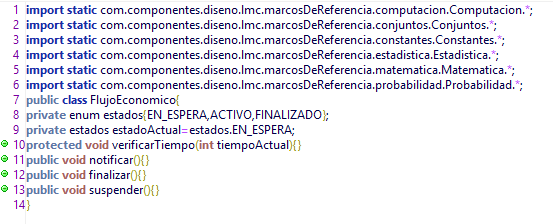
\includegraphics[width=1\linewidth]{parte2/imgs/DiagramaDeEstado/codigo}
	\caption{código de Clase Gestion Solicitud}
	\label{fig:diagramaEstadoClaseCodigo}
\end{figure}\newpage

%%%%%%%%%%%%%%%%%%%%%% Seccion 5.2 %%%%%%%%%%%%%%%%%%%%%%%%%%%%%
\section{Diagrama de flujo de trabajo}
Los diagramas de flujo de trabajo describen el comportamiento del sistema cuando tiene una actividad lo suficientemente grande para requerir un detallado de ésta, de las partes y de cómo interactuan entre sí.

Para desarrollarlo se implementan diferentes elementos como:

\begin{itemize}
	\item \textbf{Particiones}: Es una abstracción de las partes del sistema que interactua entre sí.
	\item \textbf{Actividades}: Son las tareas que le corresponde realizar a cada partición.
	\item \textbf{Transiciones}: Dan el orden en que las particiones deben desarrollar sus tareas siendo cada una dependiente de la anterior.	
	\item \textbf{Estado final}: Es el estado al que debe llegar el flujo cuando se culmine el proceso y no hayan más transiciones.
\end{itemize}

Para el software G.A.A.UD se realizo un diagrama de flujo el cual encierra las actividades fundamentales del software, iniciando desde el momento que el estudiante realiza la solicitud al apoyo alimentario hasta el momento en que es notificado si recibio dicho beneficio o no.

\paragraph{Gention de la solicitud}

 para este diagrama se requiere hacer la abtraccion de 3 paerticipantes, los cuales son el Estudiante, el Coordinador y el Revisor, iniciando desde el momento en que el estudiante realiza la solicitud, el coordinador la recive y se la envia al revisor, este la evalua luego emite dicha respuesta, la cual recive el coordinador  y segun si fue aprovada o no el coordinador le adjudicara el beneficio o no al estudiante.

\begin{figure}[H]
	\centering
	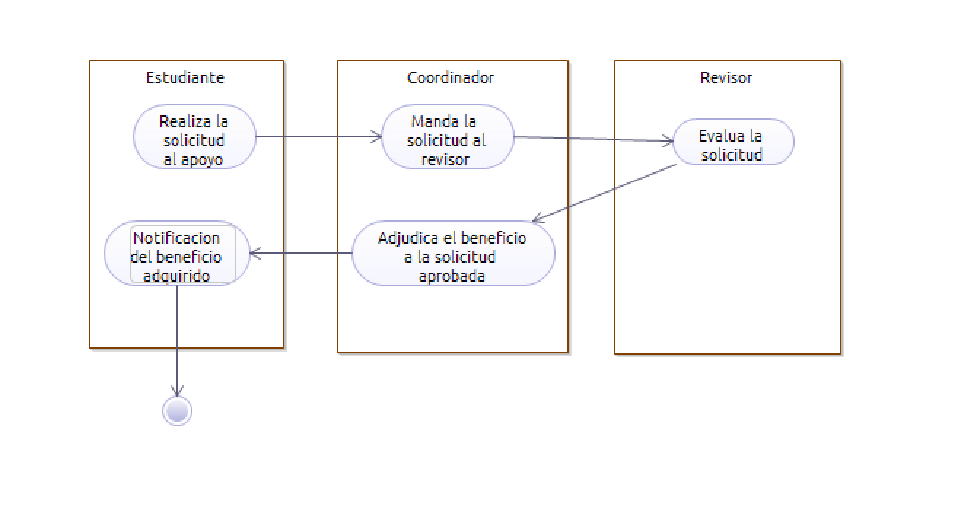
\includegraphics[width=1\linewidth]{parte2/imgs/DiagramaDeFlujoDeTrabajo/Actividades}
	\caption{Diagrama de flujo de trabajo para agregar un flujo nuevo}
	\label{fig:workflowAgregarFlujo}
\end{figure}

%Estados
%\chapterimage{metricas.jpg} % Table of contents heading image
\chapter{Diagrama de sistemas y métricas}
\section{Diagrama de sistemas}
Los diagramas de sistemas representan un concepto clave en la búsqueda de la organización y la agrupación de elementos, un ordenamiento hecho a partir de características particulares. En el lenguaje común, estos diagramas se denominan diagramas de paquetes, y dado que los paquetes contienen clases, entonces el diagrama refleja la estructura y la naturaleza del sistema en cuestión.

Los paquetes agrupan las clases de acuerdo a un parámetro de afinidad establecido por la elección del carácter del sistema, la estructura de su concepción y la organización personalizada del proyecto. Ahora bien, ese parámetro de afinidad se llama cohesión y determina el grado de correlación entre las clases para el cumplimiento del objetivo del sistema.

\begin{figure}[H]
	\centering
	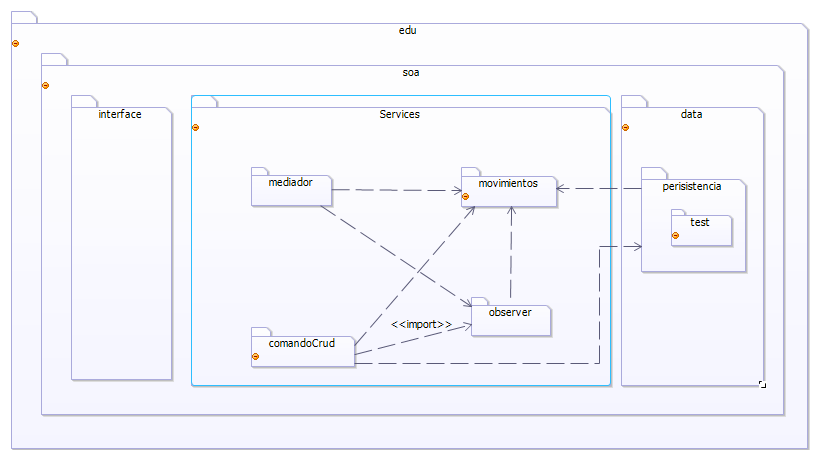
\includegraphics[width=0.9\linewidth]{parte2/imgs/DiagramaSistema/diagramaSistemas}
	\caption{Diagrama del sistema*}
	\label{fig:diagramasistemas}
\end{figure}

\begin{flushright}
	\textit{*Tanto el diagrama como los siguientes parámetros son ofrecidos por el software \textbf{Coloso}.}
\end{flushright}

Dentro de los posibles tipos de carácter que se pueden encontrar para asignarle a un proyecto esta 'com', cuándo la aplicación tiene objetivos lucrativos o comerciales, 'edu' cuando el trabajo se enmarca en cuestiones educativas, 'inv' si se involucra con investigaciones, 'gov' si entidades gubernamentales son el objetivo, entre otras. 

Existen varios tipos de arquitectura para clasificar un proyecto, dentro de los cuales se puede mencionar MVC, PAC, CORBA, SOA, de 2 niveles, de tres, etc.

Finalmente, la organización personalizada involucra de forma directa a las necesidades particulares que el proyecto requiere, por lo que no existen modelos pre-establecidos ni plantillas para usar sino que interviene el criterio personal.

El anterior diagrama de sistemas muestra la jerarquía entre paquetes, todo el proyecto encapsulado en el paquete 'edu', luego en segundo nivel de jerarquía esta la arquitectura, en este caso 'soa' ya que se busca proveer servicios desde la aplicación En la capa de datos se encuentra la persistencia, mostrada como un facade de distintos tipos de persistencia (inicialmente una de test), y requiere de clases del paquete de movimientos para estandarizar la salidas de las consultas y las entradas para actualización y creación Para el CRUD sobre la base de datos se usa el paquete comandoCrud, que trabaja sobre la forma de persistencia seleccionada, y también requiere del modulo observer ya que en cada operación sobre persistencia, y esta notifica al mediador encargado de la gestión entre flujo y sugerencias (que se encuentran el modulo movimientos). Actualmente no cuenta con salidas exteriores de interfaz.\newpage

%%%%%%%%%%%%%%%%%%% seccion 6,2 %%%%%%%%%%%%%%%%%%
\section{Métricas}
Las métricas son paramétros que establecen el nivel de calidad de un sistema, una de ellas es la inestabilidad de los paquetes y se determina a partir del grado de acoplamiento aferente (hacia afuera) y eferente (hacia adentro) de un paquete y la relación entre los mismos. Estas métricas fueron propuestas por Robert Cecil Aka en el año de 1995.

Tomando como base un paquete concreto, el acoplamiento aferente hace referencia a cuando otro paquete hace uso de atributos y/o métodos de clases de dicho paquete o hereda alguna de ellas y el acoplamiento eferente se produce cuando dicha clase hace uso de atributos y/o métodos de clases de otro paquete o hereda de clases de otro paquete.

Estas métricas relacionada con el acoplamiento surgen debido a la relación estrecha entre este, la complejidad, la mantenibilidd y la selección de clases dónde hay que prestar más atención a la hora de realizar pruebas unitarias.

Un elevado acoplamiento aferente se traduce en un paquete con un alto grado de responsabilidad. La responsabilidad y la estabilidad son dos conceptos que están unidos, esto debido a que al existir un elevado número de clases que dependen de clases del paquete, se tiene que ser más prudente a la hora de realizar modificaciones en clases del paquete, debido a los posibles efectos colaterales que se pueden generar.

El alto acoplamiento eferente tiene que ver es con un paquete con un alto grado de dependencia, término asociado con la inestabilidad ya que el funcionamiento de las clases del paquete dependen del comportamiento de clases externas, lo que las hace susceptibles de efectos colaterales en las modificaciones de las mismas y por tanto su funcionamiento encierra una mayor incertidumbre.

La inestabilidad de un paquete se representa a través de la siguiente fórmula:$$I=\frac{C_e}{C_e+C_a}$$ dónde $I$ es inestabilidad, $C_e$ es acoplamiento eferente y $C_a$ es acoplamiento aferente. Por lo tanto la inestabilidad se encontrará en un rango entre 0 y 1.

Estudiando los valores extremos podemos afirmar que si la inestabilidad de un paquete es 1 quiere decir que el acoplamiento aferente es 0 o lo que es lo mismo ninguna clase externa al paquete tiene una relación de dependencia respecto a una clase del paquete, por lo que el paquete sólo tiene dependencias hacia clases externas al paquete. El valor 1 indica una inestabilidad “extrema” del paquete (no obstante, habría que valorar también el valor individual del acoplamiento eferente, ya que, es una opinión personal mía, no todas las inestabilidad con valor 1 tendrían por qué ser iguales) ya que por un lado su comportamiento depende de clases externas, lo cual la hace posible víctima de efectos colaterales y por otro el hecho que no haya clases que dependan del paquete, da una mayor libertad a la hora de realizar modificaciones en el mismo ya que no hay que pensar en terceras clases a la hora de realizar modificaciones en el mismo (también habría que matizar esto, ya que puede haber dependencias entre clases del paquete, medibles mediante distintas métricas, que provoquen que no sea tan ágil o sencillo modificar el paquete)\cite{Pw8M}.

\paragraph{Uso de Eclipse}
Para tener una percepción más visual sobre las métricas de nuestro programa, acudimos al software ECLIPSE, dado que en éste vamos a programar nuestras clases y paquetes, y con ayuda de un plúgin especializado en métricas llamado STAN, hallamos los diagramas de composición, de polución y una grafica de distancia entre inestabilidad y abstracción.

\paragraph{Diagramas de Composición}

La vista de composición permite mirar en el artefacto seleccionado, para ver todos sus contenidos y las dependencias entre ellos. Puede investigar dependencias entre miembros de una clase, clases de un paquete, paquetes, hijos de un árbol de paquetes y entre librerías\cite{Pw9Cmp}.

\begin{figure}[H]
	\centering
	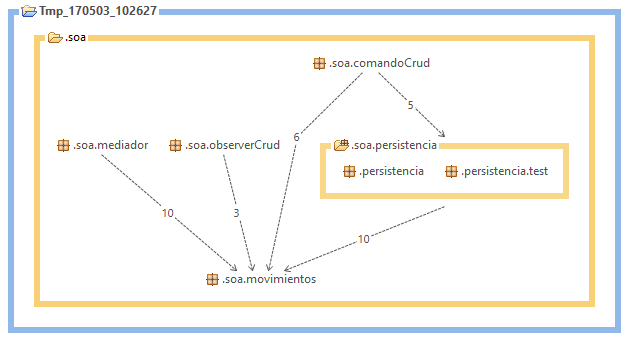
\includegraphics[width=1\linewidth]{parte2/imgs/Metricas/diagramaComposicion}
	\caption{Diagrama de composición del sistema}
	\label{fig:composicion}
\end{figure}

Dado que se puede navegar por cualquiera de los artefactos mostrados, a  continuación mostraremos los diagramas de composición de cada paquete.

\begin{figure}[H]
	\centering
	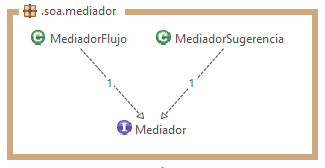
\includegraphics[width=0.7\linewidth]{parte2/imgs/Metricas/SoaMediador}
	\caption{Diagrama de composición del paquete mediador}
	\label{fig:soamediador}
\end{figure}

\begin{figure}[H]
	\centering
	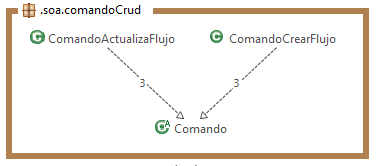
\includegraphics[width=0.7\linewidth]{parte2/imgs/Metricas/SoaComandoCrud}
	\caption{Diagrama de composición del paquete comando}
	\label{fig:soacomandocrud}
\end{figure}

\begin{figure}[H]
	\centering
	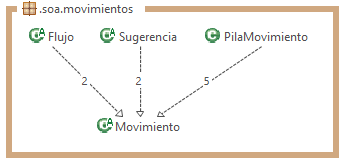
\includegraphics[width=0.7\linewidth]{parte2/imgs/Metricas/SoaMovimientos}
	\caption{Diagrama de composición del paquete Movimientos}
	\label{fig:soamovimientos}
\end{figure}

\begin{figure}[H]
	\centering
	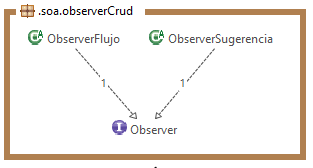
\includegraphics[width=0.5\linewidth]{parte2/imgs/Metricas/SoaObserverCrud}
	\caption{Diagrama de composición del paquete ObseverCrud}
	\label{fig:soaobservercrud}
\end{figure}

\begin{figure}[H]
	\centering
	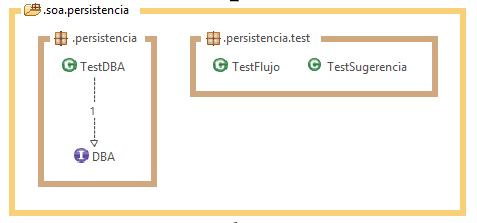
\includegraphics[width=0.7\linewidth]{parte2/imgs/Metricas/SoaPersistencia}
	\caption{Diagrama de composición del paquete de Persistencia}
	\label{fig:soapersistencia}
\end{figure}

\paragraph{Diagrama de Polución}

Un artefacto se dice que viola una métrica si se califica ámbar o rojo para esa métrica. Para cada artefacto, STAN muestra todas las métricas que son violadas por el propio artefacto o por artefactos contenidos.

STAN asume que las violaciones en artefactos "grandes" son peores que las violaciones en "pequeñas": debería ser más relevante si un paquete recibió una mala calificación para alguna métrica A que si una de sus 42 clases recibió una calificación similar para alguna métrica B .Además, incluso si un paquete es calificado ámbar para A, esto podría ser más relevante que si una de sus clases tiene un valor rojo para B\cite{Pw10V&P}.

Para tener esto en cuenta, STAN prioriza una infracción métrica ponderando su clasificación con la cantidad del código subyacente del artefacto. El resultado se muestra en la vista Violaciones.

\begin{figure}[H]
	\centering
	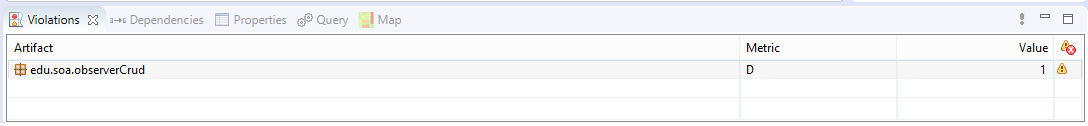
\includegraphics[width=0.8\linewidth]{parte2/imgs/Metricas/violaciones}
	\caption{Violaciones de los artefactos del sistema}
	\label{fig:violaciones}
\end{figure}

Por último, para un determinado artefacto, es posible que desee obtener una idea de cómo las métricas contribuyen a sus violaciones y lo mal que el artefacto está contaminado por las violaciones. Ésto se puede ver el gráfico de contaminación o polución de STAN, en el cual,Cuanto más ancho sea el anillo, mayor será el grado de contaminación del código subyacente. En el nivel de aplicación, el espesor del anillo puede servir como indicador rápido de la calidad estructural global de la base de código\cite{Pw10V&P}.

A continuación podemos ver el diagrama de polución para el sistema: 

\begin{figure}[H]
	\centering
	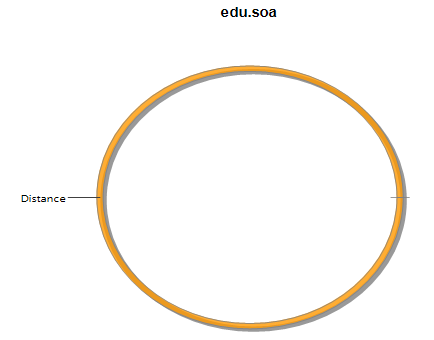
\includegraphics[width=0.6\linewidth]{parte2/imgs/Metricas/diagramaPolucion}
	\caption{Diagrama de polución del sistema}
	\label{fig:polucion}
\end{figure}

\begin{figure}[H]
	\centering
	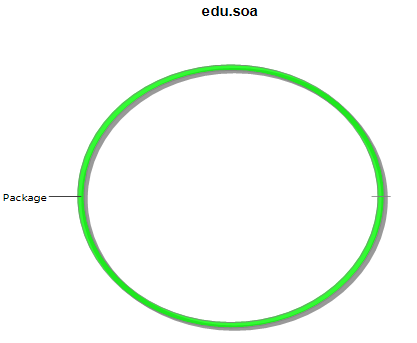
\includegraphics[width=0.6\linewidth]{parte2/imgs/Metricas/diagramaPolucionDominio}
	\caption{Diagrama de polución del sistema según los paquetes}
	\label{fig:polucionDominio}
\end{figure}

Dado que el único artefacto que tiene una violación es el paquete de ObserverCrud, es imprescindible visualizar la polución de éste:

\begin{figure}[H]
	\centering
	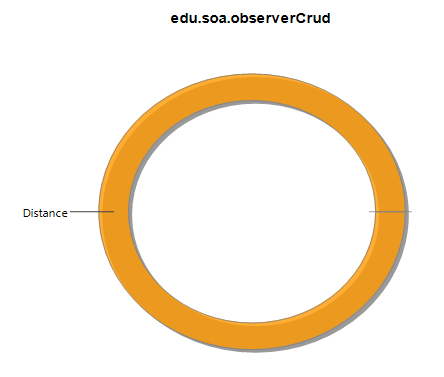
\includegraphics[width=0.6\linewidth]{parte2/imgs/Metricas/diagramaPolucionObserver}
	\caption{Diagrama de polución del paquete ObserverCrud}
	\label{fig:diagramapolucionobserver}
\end{figure}

\begin{figure}[H]
	\centering
	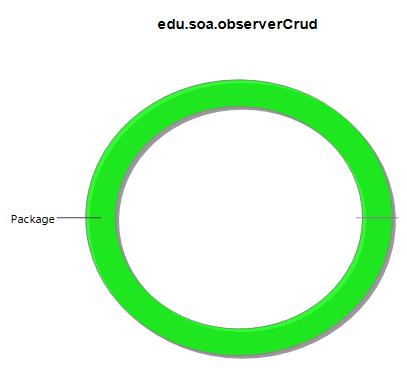
\includegraphics[width=0.6\linewidth]{parte2/imgs/Metricas/diagramaPolucionDominioObserver}
	\caption{Diagrama de polución del paquete ObserverCrud según los paquetes}
	\label{fig:diagramapoluciondominioobserver}
\end{figure}

\paragraph{Grafica de distancia}

Robert C. Martin propuso la idea de que para un software bien diseñado debe haber una relación específica entre dos medidas de paquete: la abstracción de un paquete, que expresará la porción de tipos abstractos contenidos, y su estabilidad, que indica si el paquete es principalmente Utilizado por otros artefactos (estable) o si depende principalmente de otros artefactos (inestables)\cite{Pw11D}.

La relación deseada se captura en el principio de abstracción estable : Un paquete debe ser tan abstracto como estable.

Siguiendo este principio, evitamos obtener paquetes que son utilizados en gran medida por el resto de la aplicación y que, al mismo tiempo, tienen un bajo grado de abstracción. Estos paquetes son una fuente constante de problemas, ya que son difíciles de cambiar o extender.

\begin{itemize}
	\item \textbf{La Abstracción} A para el paquete P se calcula como la relación entre el número de tipos abstractos contenidos en P y el número total de tipos en P. Así, los valores resultantes van desde cero (sólo clases concretas) a uno (sólo interfaces y clases abstractas).
	\item \textbf{La Inestabilidad} I para el paquete P se calcula como la relación entre el número de clases fuera de P requerido por P y el número total de clases fuera de P relacionadas con P. Como anteriormente, los valores resultantes van desde cero (sólo dependencias entrantes) a uno (sólo dependencias salientes).
\end{itemize}

Así que ahora tenemos todo junto para definir la Distancia D , que indica cuán lejos está un paquete de la Secuencia Principal:

$$D=A+I-1$$

Calculando la distancia de esta manera, obtenemos valores entre -1 y 1. Un valor cero significa que el paquete se encuentra exactamente en la Diagonal Principal, el signo indica si el paquete se encuentra por encima o por debajo de la Secuencia Principal. Una métrica derivada, la Distancia Absoluta (| D |), omite el signo, permitiendo así calcular valores medios significativos para artefactos de mayor nivel.

La tabla de distancias STAN le muestra dónde están sus paquetes en vivo, si están ubicados cerca de la Secuencia Principal, como se desee, o si tienden a deslizarse hacia las malas esquinas. Cada paquete se muestra mediante una burbuja, cuyo tamaño está determinado por el número de clases del paquete. El color de la burbuja refleja la clasificación del valor de distancia del paquete, que es, como siempre, ajustable a sus necesidades\cite{Pw11D}.

La siguiente es la distancia de nuestros paquetes en la gráfica de STAN:S

\begin{figure}[H]
	\centering
	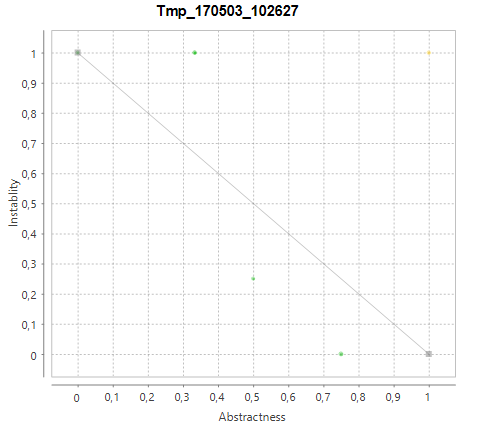
\includegraphics[width=0.7\linewidth]{parte2/imgs/Metricas/diagramaDistancia}
	\caption{Diagrama de distancia del sistema}
	\label{fig:distancia}
\end{figure} %metricas
%\chapterimage{componentes.jpg} % Table of contents heading image
\chapter{Componentes}

Se define componente como el medio a través del cual se realiza una encapsulación a un nivel mayor al de una clase o un paquete, de forma que se introduzcan allí soluciones, y se exporten a través de interfaces, lo cual construye un ecosistema de interacción a través de elementos denominados cajas negras, aquellas con las cuales solo es posible la interacción y no la modificación, todo encaminado a brindar de una mayor seguridad a los módulos Estos componentes son parte de un sistema o un subsistema del mismo. El sistema puede estar formado por uno o varios de éstos. Se tratan de elementos que, a través de algún tipo de asociación o contigüidad, dan lugar a un conjunto uniforme.\nocite{Notas}

Para una aplicación los componentes funcionan como cajas negras, los cuales son elementos que reciben una entrada y según ésta, dan una respuesta de salida sin tener en cuenta cómo es su funcionamiento interno, en otras palabras, de una caja negra será primordial la forma en que interactua con el medio que existe sin hacer relevante los procesos que llevan a cabo.

La implementación de componentes como parte del sistema se hace para evitar que se ha denominado aplicación monolítica, dado que esta describe una única aplicación de software en niveles en los que la interfaz de usuario y código de acceso a datos se combinan en un solo programa de una plataforma única \cite{Pw6AM}.

Las Aplicaciones monolíticas aunque se pueden desarrollar sin problema alguno, tienen bastantes desventajas como por ejemplo:

\begin{itemize}
		\item Requieren mayor hardware en las estaciones de trabajo
		\item Son infinitamente más lentos en el procesamiento de peticiones sencillas
		\item Requiere habilitar el acceso real a la carpeta de datos para todos los usuarios de la aplicación 
		\item Su actualización es más costosa
		\item No permite el acceso en línea desde fuera de la red local o requieren de implementaciones de soluciones de conectividad muy costosa.
		\item Ocupan mayor ancho de banda, provocando congestionamiento en la Red Local.
\end{itemize}

Por esto mismo se tiene como preferencia que las diferentes soluciones se caractericen por la mayor cantidad de componentes como sean requeridos.

\section{Diagrama de componentes}

Un diagrama de componentes es un diagrama de tipo del Lenguaje Unificado de Modelado (UML). Éste representa cómo un sistema de software es dividido en componentes y muestra la interacción entre estos componentes.

Un diagrama de componentes muestra los elementos de un diseño de un sistema de software, permite visualizar la estructura de alto nivel del sistema y el comportamiento del servicio que estos componentes proporcionan y usan a través de interfaces\cite{Pw7DC}.

Para entender estos diagramas, es necesario definir los elementos que posee:
\begin{itemize}
	\item \textbf{Componentes}: Es una parte física del sistema, ya sea un modulo, base de datos, programa externo,etc. 
	\item \textbf{Interfaces}: Es el lazo de unión de varios componentes, puede ser requerida, en cuyo caso representa un grupo de mensajes o llamadas que envía el componente a otros componentes o sistemas externos la cual está diseñada para acoplarse a componentes que proporcionan estas operaciones, o ser proveída, por lo que son aquellas llamadas o mensajes que implementa un componente y puede ser usada por otros componentes o sistemas externos. En general estas interfaces son las que definen el api del componente.
	\item \textbf{Paquetes o sub-sistemas}: Algunas veces varios componentes pueden agruparse en un solo paquete o venir dentro de otros componentes que funcionen como sub-sistemas.
\end{itemize} 

Para nuestra aplicación se han desarrollado conco componentes para su funcionamiento, se han definido los siguientes componentes, AppPrincipal, EnvioCorreos, VerificarEstudiantes, VerificarConvocatoria, AgregarBeneficios.

\begin{figure}[H]
	\centering
	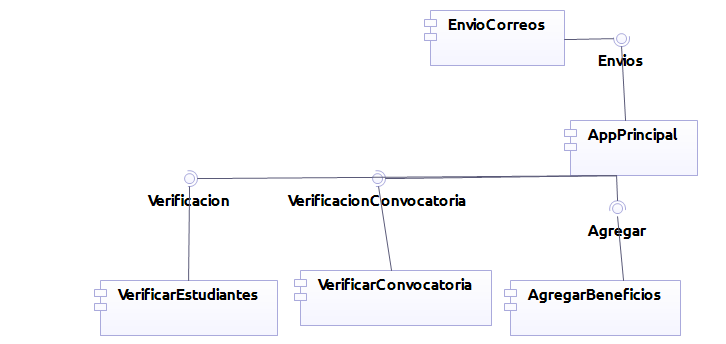
\includegraphics[width=1\linewidth]{parte2/imgs/DiagramaDeComponentes/componentes}
	\caption{Diagrama de componentes }
	\label{fig:api}
\end{figure}

Para un mayor detalle de cómo funcionan los componentes seleccionados, en la siguiente figura se puede visualizar un diagrama de clases para cada uno de forma particular.

\begin{figure}[H]
	\centering
	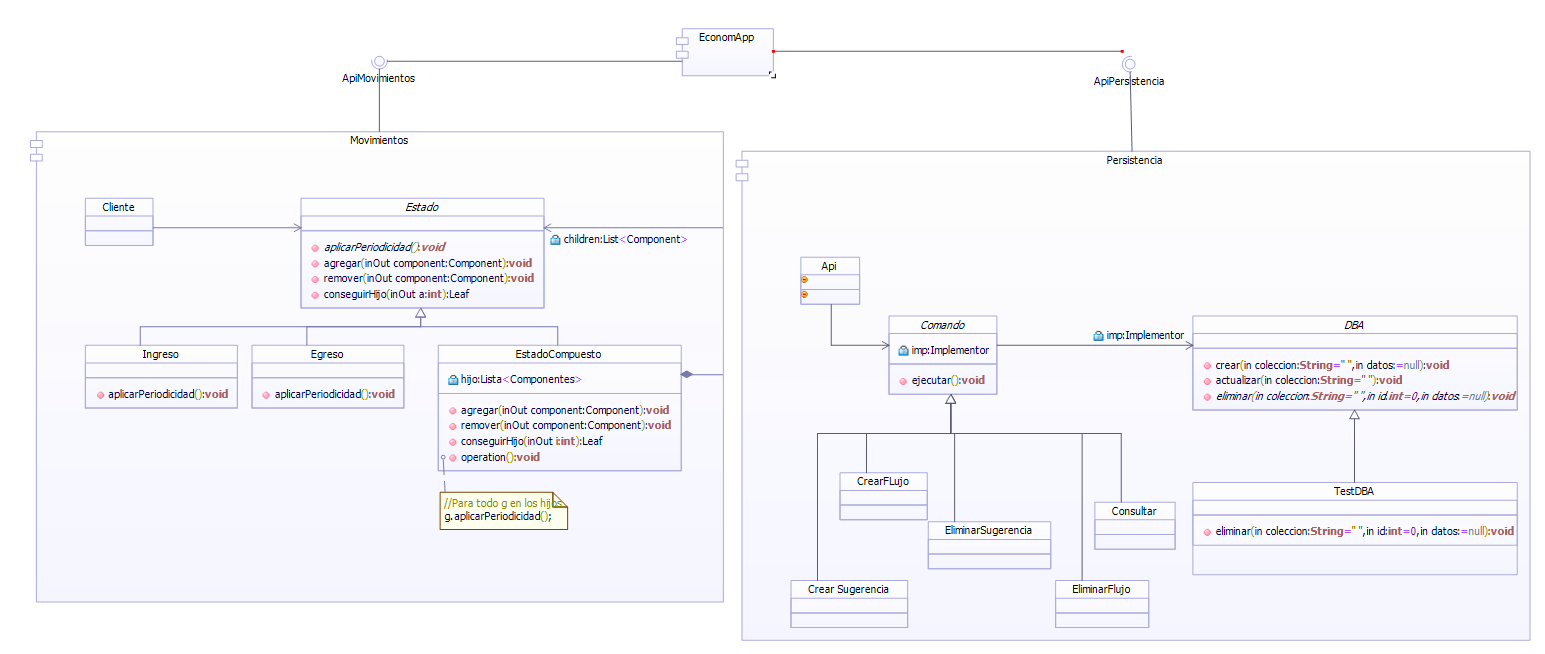
\includegraphics[width=1\linewidth]{parte2/imgs/DiagramaDeComponentes/apiDetallado}
	\caption{Detallado de la estructura interna de los componentes}
	\label{fig:apidetallado}
\end{figure}

Así, el componente de Movimientos se fundamenta en el patrón de Estado, en éste se define la interacción y el cambio de estado de los elementos con los que funcionará el programa, como lo son INGRESO y EGRESO, los cuales heredan de estado. 	

Mientras que en el componente de persistencia se puede apreciar la implementación del patrón Comando, en este componente se manejara todo el tema relacionado con la persistencia del programa, es decir, la base de datos de la que dispone, utilizando el patrón comando para gestionar el CRUD de la base de datos de forma eficiente.  %componentes
%\chapterimage{conclusiones.jpg} % Table of contents heading image
\chapter{Conclusiones, Trabajos Futuros}

\section{Conclusiones}
Después de realizar el recorrido a lo largo del estudio de los procesos y metodologías de software, y además, mirar las estructuras que definían el diseño de software para luego implementarlo en el proyecto del curso, fue posible realizar las siguientes conclusiones:
\begin{itemize}
	\item El desarrollo de software se basa esencialmente en la definición y posterior ejecución de tres grandes aspectos: la especificación, el desarrollo y el mantenimiento. Estos grandes pilares representan la base a la hora de emprender cualquier proyecto de software y se encuentran en cualquiera de los posibles caminos que especifique una metodología, ya sea de forma explícita o implícitamente.  
	
	\item A lo largo de los años se han venido construyendo propuestas sobre las cuales trabajar para poder fijar el rumbo de un proyecto, todas siempre sustentadas en la experiencia y que tienen en cuenta situaciones específicas. Para el proyecto particular de EcnonomApp, el hecho de haber escogido la metodología RUP fue precisamente debido a que sus protocolos se ajustaban a las necesidades de la construcción de la aplicación, es decir, la capacidad de no tener estados rígidos y dependientes sino una serie de procesos adaptables, prioridades balanceadas, adquisición de valor de forma iterativa, entre otras, se ajustaban a las necesidades del equipo.
	
	\item Una vez establecida la forma en la que se realizan las cosas llega la hora de trabajarlas. Es allí donde la definición de requerimientos adquiere una importancia natural, porque fija el punto de partida, señala lo que el sistema final debe realizar, establece una característica de rendimiento con la cual evaluar el resultado, y desde la cual establecer las correcciones necesarias llegado el caso que no se logre lo esperado.
	
	\item El lenguaje UML proporciona una serie de herramientas estandarizadas que se ofrecen con el fin de realizar una explicación asertiva del sistema al cual hace referencia, por lo que brinda la capacidad de que cualquier persona, incluso que no se halla encontrado en la construcción de un proyecto, lo entienda e interprete.
	
	\item El objetivo del lenguaje UML es la respuesta al ¿cómo? del sistema, una vez expuesto el ¿qué? en el establecimiento de los requerimientos y los casos de uso. Para empezar a describir el ¿cómo? se empieza desde la parte de la identificación de objetos y su comunicación, esto no es de extrañar dado que UMl nace en el marco del paradigma de la programación orientada a objetos.
	
	\item Después de las posterior generalización de los objetos en clases, surgen conceptos. Dentro de la especificación de los pilares de la orientación a objetos se habla de que los programas deben ser abiertos para la extensión y cerrados para la modificación, es allí donde nacen dos conceptos completamente nuevos, y son las cajas blancas y las cajas negras, donde las primeras son abstracciones encaminadas a un acoplamiento máximo y una seguridad mínima, y las segundas ofrecen seguridad máxima y acoplamiento mínimo.
	
	\item En el diseño de los programas se mide el nivel de confianza de una estructura pensada en función del número de interfaces y clases abstractas que contenga, por lo que si se visualizan exceso de clases concretas, es necesario preocuparse por la forma como se modeló el problema.
	
	\item Muchas veces un elemento en el contexto del diseño de sotware sufre cambios en su estado, los cuales afectan de forma directa el comportamiento de éste y su uso en determinadas situaciones. Es por ello que se utiliza el diagrama de máquina de estados, para visualizar la interacción entre diferentes estados a partir de disparos y transiciones.
	
	\item En un sistema es importante poder visualizar el flujo de algún elemento y la señalización del paso de una actividad a otra, es decir los procesos en alto nivel, es por ello que se utiliza el diagrama de actividades, y es allí donde recae su importancia.
	
	\item Llegando al final del diseño uno de los temas que va aumentando su nivel de complejidad es el de la agrupación y la organización de modulos, empezando por el concepto de sistemas dónde se analiza una característica principal y un grado alto de afinidad modular para segmentar y clasificar las clases y guardarlas en paquetes. Después, pasando por el concepto de componentes en los cuales se busca cual es el trabajo de determinados sistemas y se procede a segmentarlos en unidades aún mas diferenciables, y que además tengan capacidades de ser coherentes en sí mismos, es decir, no depender de ninguna otra instancia para poder saber cual es su función. Finalmente, se llega al concepto de nodo, en el cual, desde un punto de vista más alejado del software y mas general, se corresponde a poner determinados sistemas en deterinados nodos dependiendo de cual es el recurso que éstos necesitan.
	
	\item Todos estos aspectos se utilizan para poder hacer frente de una forma especializada a la dificil tarea de la construcción de soluciones, pero gracias a las buenas prácticas de diseño, se simplifica de forma que sea un aspecto manejable y posible, aterrizando todos los experimentos reales en una cuestión práctica, concreta y tangible.
\end{itemize}
\section{Trabajos Futuros}
El objetivo del proyecto era la construcción de una aplicación de economía personal. El prototipo logrado llega hasta la parte del ingreso de movimientos y flujos, del registro de una persona y la visualización de sus datos. Como trabajo futuro se espera lograr una especificación precisa de todas las variables que intervienen en el ejercicio de la economía, por lo tanto una versión posterior lograría tomar todas las variables y fijar la importancia de estas en función de generar resultados más precisos. Además en un trabajo futuro se podría incluir la opción de asociar una tarjeta débito o crédito para automatizar algunas tareas con datos de los bancos asociados a dichos medios. Otra de las posibles características a incluir podría ser la realización de sugerencias de qué cosas comprar y dónde conseguirlas gracias a las capacidades que brinda internet para la búsqueda de artículos en línea, entre otros. %diagrama de nodos

\part{Reflexiones}
\chapterimage{conclusiones.jpg} % Table of contents heading image
\chapter{Conclusiones, Trabajos Futuros}

\section{Conclusiones}
Después de realizar el recorrido a lo largo del estudio de los procesos y metodologías de software, y además, mirar las estructuras que definían el diseño de software para luego implementarlo en el proyecto del curso, fue posible realizar las siguientes conclusiones:
\begin{itemize}
	\item El desarrollo de software se basa esencialmente en la definición y posterior ejecución de tres grandes aspectos: la especificación, el desarrollo y el mantenimiento. Estos grandes pilares representan la base a la hora de emprender cualquier proyecto de software y se encuentran en cualquiera de los posibles caminos que especifique una metodología, ya sea de forma explícita o implícitamente.  
	
	\item A lo largo de los años se han venido construyendo propuestas sobre las cuales trabajar para poder fijar el rumbo de un proyecto, todas siempre sustentadas en la experiencia y que tienen en cuenta situaciones específicas. Para el proyecto particular de EcnonomApp, el hecho de haber escogido la metodología RUP fue precisamente debido a que sus protocolos se ajustaban a las necesidades de la construcción de la aplicación, es decir, la capacidad de no tener estados rígidos y dependientes sino una serie de procesos adaptables, prioridades balanceadas, adquisición de valor de forma iterativa, entre otras, se ajustaban a las necesidades del equipo.
	
	\item Una vez establecida la forma en la que se realizan las cosas llega la hora de trabajarlas. Es allí donde la definición de requerimientos adquiere una importancia natural, porque fija el punto de partida, señala lo que el sistema final debe realizar, establece una característica de rendimiento con la cual evaluar el resultado, y desde la cual establecer las correcciones necesarias llegado el caso que no se logre lo esperado.
	
	\item El lenguaje UML proporciona una serie de herramientas estandarizadas que se ofrecen con el fin de realizar una explicación asertiva del sistema al cual hace referencia, por lo que brinda la capacidad de que cualquier persona, incluso que no se halla encontrado en la construcción de un proyecto, lo entienda e interprete.
	
	\item El objetivo del lenguaje UML es la respuesta al ¿cómo? del sistema, una vez expuesto el ¿qué? en el establecimiento de los requerimientos y los casos de uso. Para empezar a describir el ¿cómo? se empieza desde la parte de la identificación de objetos y su comunicación, esto no es de extrañar dado que UMl nace en el marco del paradigma de la programación orientada a objetos.
	
	\item Después de las posterior generalización de los objetos en clases, surgen conceptos. Dentro de la especificación de los pilares de la orientación a objetos se habla de que los programas deben ser abiertos para la extensión y cerrados para la modificación, es allí donde nacen dos conceptos completamente nuevos, y son las cajas blancas y las cajas negras, donde las primeras son abstracciones encaminadas a un acoplamiento máximo y una seguridad mínima, y las segundas ofrecen seguridad máxima y acoplamiento mínimo.
	
	\item En el diseño de los programas se mide el nivel de confianza de una estructura pensada en función del número de interfaces y clases abstractas que contenga, por lo que si se visualizan exceso de clases concretas, es necesario preocuparse por la forma como se modeló el problema.
	
	\item Muchas veces un elemento en el contexto del diseño de sotware sufre cambios en su estado, los cuales afectan de forma directa el comportamiento de éste y su uso en determinadas situaciones. Es por ello que se utiliza el diagrama de máquina de estados, para visualizar la interacción entre diferentes estados a partir de disparos y transiciones.
	
	\item En un sistema es importante poder visualizar el flujo de algún elemento y la señalización del paso de una actividad a otra, es decir los procesos en alto nivel, es por ello que se utiliza el diagrama de actividades, y es allí donde recae su importancia.
	
	\item Llegando al final del diseño uno de los temas que va aumentando su nivel de complejidad es el de la agrupación y la organización de modulos, empezando por el concepto de sistemas dónde se analiza una característica principal y un grado alto de afinidad modular para segmentar y clasificar las clases y guardarlas en paquetes. Después, pasando por el concepto de componentes en los cuales se busca cual es el trabajo de determinados sistemas y se procede a segmentarlos en unidades aún mas diferenciables, y que además tengan capacidades de ser coherentes en sí mismos, es decir, no depender de ninguna otra instancia para poder saber cual es su función. Finalmente, se llega al concepto de nodo, en el cual, desde un punto de vista más alejado del software y mas general, se corresponde a poner determinados sistemas en deterinados nodos dependiendo de cual es el recurso que éstos necesitan.
	
	\item Todos estos aspectos se utilizan para poder hacer frente de una forma especializada a la dificil tarea de la construcción de soluciones, pero gracias a las buenas prácticas de diseño, se simplifica de forma que sea un aspecto manejable y posible, aterrizando todos los experimentos reales en una cuestión práctica, concreta y tangible.
\end{itemize}
\section{Trabajos Futuros}
El objetivo del proyecto era la construcción de una aplicación de economía personal. El prototipo logrado llega hasta la parte del ingreso de movimientos y flujos, del registro de una persona y la visualización de sus datos. Como trabajo futuro se espera lograr una especificación precisa de todas las variables que intervienen en el ejercicio de la economía, por lo tanto una versión posterior lograría tomar todas las variables y fijar la importancia de estas en función de generar resultados más precisos. Además en un trabajo futuro se podría incluir la opción de asociar una tarjeta débito o crédito para automatizar algunas tareas con datos de los bancos asociados a dichos medios. Otra de las posibles características a incluir podría ser la realización de sugerencias de qué cosas comprar y dónde conseguirlas gracias a las capacidades que brinda internet para la búsqueda de artículos en línea, entre otros.%conclusiones
\chapterimage{anexos.jpg} % Table of contents heading image
\chapter{Anexos}
\section{Código de los patrones}
\subsection{Patron Estado}
\lstinputlisting[language=TypeScript]{codigo/Patrones/Estado.ts}
%\lstinputlisting[language=TypeScript]{codigo/index.ts}
\clearpage
\subsection{Patron Builder}
\lstinputlisting[language=TypeScript]{codigo/Patrones/Builder.ts}
\subsection{Patron Singleton}
\lstinputlisting[language=TypeScript]{codigo/Patrones/Singleton.ts}

\subsection{Patron Iterador}
\lstinputlisting[language=TypeScript]{codigo/Patrones/Iterator.ts}
% codigo

%BIBLIOGRAFÍA
\chapterimage{referencias.jpg} % Table of contents heading image
\printbibliography%Mostrar Bibliografía
\end{document}